\documentclass[conference]{IEEEtran}

% ---------------------------------------------------------------------------
% Abstracts must be submitted by August 10-12th; submitted abstracts may not
% exceed 500 words. submitted
% manuscripts may not exceed ten (10) single-spaced double-column pages using
% 10-point size font on 8.5x11 inch pages (IEEE conference style), including
% figures, tables, and references. The submitted manuscripts should include
% author names and affiliations. The submission portal will be available by
% September. Return to this site to submit your abstract and upload your
% submissions.
% ---------------------------------------------------------------------------

%\usepackage[numbers, sort, compress]{natbib}
\usepackage{graphicx}
\usepackage{amsmath}
\usepackage{amssymb}
\usepackage{color}
\usepackage{ifpdf}
%\usepackage{mdwlist}

%\usepackage{dcolumn}
\usepackage{float}
\usepackage[utf8]{inputenc}
\usepackage{multirow}
\usepackage{rotating}
% DEPRECATED!
%\usepackage{subfigure}
\usepackage[caption=false]{subfig}

\usepackage{moresize}
%\usepackage{setspace}

%\usepackage[numbers, sort, compress]{natbib}
%\usepackage{latex8}
%\usepackage{float}
%\usepackage{times}
\usepackage[hyphens]{url}
\usepackage{booktabs}
\usepackage{listings}
\usepackage{paralist}
\usepackage{wrapfig}
%\usepackage[footnotesize,it]{caption}
\usepackage{multirow}
\usepackage{ifpdf}
%\usepackage{srcltx}
\usepackage{xspace}
\usepackage{keyval}
\usepackage{color}
\usepackage{soul}

%\usepackage{draftwatermark}
%\SetWatermarkLightness{0.8}
%\SetWatermarkText{Draft}
%\SetWatermarkVerCenter{13cm}
%\SetWatermarkHorCenter{10cm}
%\SetWatermarkScale{1}

\usepackage{comment}

\definecolor{listinggray}{gray}{0.95}
\definecolor{darkgray}{gray}{0.7}
\definecolor{commentgreen}{rgb}{0, 0.4, 0}
\definecolor{darkblue}{rgb}{0, 0, 0.4}
\definecolor{middleblue}{rgb}{0, 0, 0.7}
\definecolor{darkred}{rgb}{0.4, 0, 0}
\definecolor{brown}{rgb}{0.5, 0.5, 0}
\definecolor{dkgreen}{rgb}{0,0.5,0}
\definecolor{orange}{rgb}{1,.5,0}
\definecolor{dandelion}{cmyk}{0,0.29,0.84,0}

\usepackage[normalem]{ulem}
\makeatletter
\def\cyanuwave{\bgroup \markoverwith{\lower3.5\p@\hbox{\sixly \textcolor{cyan}{\char58}}}\ULon}
\def\reduwave{\bgroup \markoverwith{\lower3.5\p@\hbox{\sixly \textcolor{red}{\char58}}}\ULon}
\def\blueuwave{\bgroup \markoverwith{\lower3.5\p@\hbox{\sixly \textcolor{blue}{\char58}}}\ULon}
\font\sixly=lasy6 % does not re-load if already loaded, so no memory problem.
\makeatother

\let\labelindent\relax
\usepackage{enumitem}

%\usepackage{xcolor}

\newif\ifdraft
\drafttrue
\ifdraft
 \newcommand{\N}[1]{\textbf{*** NOTE: #1}\xspace}
 \newcommand{\jhanote}[1]{ {\textcolor{red} { ***SJ: #1 }}}
 \newcommand{\mtnote}[1]{ {\textcolor{orange} { ***MT: #1 }}}
 \newcommand{\note}[1]{ {\textcolor{brown} { *** #1 }}}
 \newcommand{\jdnote}[1]{ {\textcolor{cyan} { ***JD: #1 }}}
 \newcommand{\dwwnote}[1]{ {\textcolor{blue} { ***DWW: #1 }}}
\else
 \newcommand{\N}[1]{}
 \newcommand{\jhanote}[1]{}
 \newcommand{\mtnote}[1]{}
 \newcommand{\jdnote}[1]{}
 \newcommand{\dwwnote}[1]{}
 \newcommand{\note}[1]{}
\fi

\newcommand{\cloud}{cloud\xspace}
\newcommand{\clouds}{clouds\xspace}
\newcommand{\pilot}{Pilot\xspace}
\newcommand{\pilots}{Pilots\xspace}
\newcommand{\pilotjob}{Pilot-Job\xspace}
\newcommand{\pilotjobs}{Pilot-Jobs\xspace}
\newcommand{\pilotcompute}{Pilot-Compute\xspace}
\newcommand{\pilotcomputedescription}{Pilot-Compute Description\xspace}
\newcommand{\pilotdescription}{Pilot-Description\xspace}
\newcommand{\pilotcomputes}{Pilot-Computes\xspace}
\newcommand{\pilotdata}{Pilot-Data\xspace}
\newcommand{\pilotdatadescription}{Pilot-Data Description\xspace}
\newcommand{\pilotdataservice}{Pilot-Data Service\xspace}
\newcommand{\pilotcomputeservice}{Pilot-Compute Service\xspace}
\newcommand{\computedataservice}{Compute-Data Service\xspace}
\newcommand{\computeunitdescription}{Compute-Unit Description\xspace}
\newcommand{\dataunitdescription}{Data-Unit Description\xspace}
\newcommand{\pilotmapreduce}{PilotMapReduce\xspace}
\newcommand{\mrmg}{MR-Manager\xspace}
\newcommand{\pstar}{P*\xspace}
\newcommand{\pd}{PD\xspace}
\newcommand{\pc}{PC\xspace}
\newcommand{\pcs}{PCs\xspace}
\newcommand{\pj}{PJ\xspace}
\newcommand{\pjs}{PJs\xspace}
\newcommand{\pds}{Pilot Data Service\xspace}
\newcommand{\computeunit}{Compute-Unit\xspace}
\newcommand{\computeunits}{Compute-Units\xspace}
\newcommand{\dataunit}{Data-Unit\xspace}
\newcommand{\dataunits}{Data-Units\xspace}
\newcommand{\du}{DU\xspace}
\newcommand{\dus}{DUs\xspace}
\newcommand{\dud}{DUD\xspace}
\newcommand{\cu}{CU\xspace}
\newcommand{\cus}{CUs\xspace}
\newcommand{\cud}{CUD\xspace}
\newcommand{\su}{SU\xspace}
\newcommand{\sus}{SUs\xspace}
\newcommand{\schedulableunit}{Schedulable Unit\xspace}
\newcommand{\schedulableunits}{Schedulable Units\xspace}
\newcommand{\cc}{c\&c\xspace}
\newcommand{\CC}{C\&C\xspace}
\newcommand{\up}{\vspace*{-1em}}
\newcommand{\upp}{\vspace*{-0.5em}}
\newcommand{\numrep}{8 }
\newcommand{\samplenum}{4 }
\newcommand{\tmax}{$T_{max}$ }
\newcommand{\tc}{$T_{C}$ }
\newcommand{\tcnsp}{$T_{C}$}
\newcommand{\bj}{BigJob\xspace}
\newcommand{\irods}{iRODS\xspace}

\newcommand{\I}[1]{\textit{#1}\xspace}
\newcommand{\B}[1]{\textbf{#1}\xspace}
\newcommand{\T}[1]{\texttt{#1}\xspace}
%\newcommand{\C}[1]{\textsc{#1}\xspace}

\newcommand{\mr}[1]{\multirow{2}{*}{#1}}%
\newcommand{\mc}[2]{\multicolumn{#1}{l}{#2}}

\lstdefinestyle{myListing}{
  frame=single,
  backgroundcolor=\color{listinggray},
  %float=t,
  language=C,
  basicstyle=\ttfamily \footnotesize,
  breakautoindent=true,
  breaklines=true
  tabsize=2,
  captionpos=b,
  aboveskip=0em,
  belowskip=-2em,
  %numbers=left,
  %numberstyle=\tiny
}

\lstdefinestyle{myPythonListing}{
  frame=single,
  backgroundcolor=\color{listinggray},
  %float=t,
  language=Python,
  basicstyle=\ttfamily \scriptsize,
  breakautoindent=true,
  breaklines=true
  tabsize=2,
  captionpos=b,
  %numbers=left,
  %numberstyle=\tiny
}



%  \setlength{\parskip}{0.05ex} % 1ex plus 0.5ex minus 0.2ex}
%  \setlength{\parsep}{0pt}
%  %\setlength{\headsep}{0pt}
%  \setlength{\topskip}{0pt}
%  \setlength{\topmargin}{0pt}
%  %\setlength{\topsep}{0pt}
%  \setlength{\partopsep}{0pt}

% This is now the recommended way for checking for PDFLaTeX:


\ifpdf
\DeclareGraphicsExtensions{.pdf, .jpg, .tif}
\else
\DeclareGraphicsExtensions{.ps,  .eps, .jpg}
\fi

\tolerance=1000
\hyphenpenalty=10


% \keywords{Distributed computing, Workload management system}

\usepackage{draftwatermark}
\SetWatermarkText{DRAFT}
\SetWatermarkScale{1}

% ---------------------------------------------------------------------------
% BEGIN DOCUMENT
% ---------------------------------------------------------------------------
\begin{document}

\title{High-throughput Binding Affinity Calculations at Extreme Scales}

\author{
    \IEEEauthorblockA{
    }
    \IEEEauthorblockA{
        \IEEEauthorrefmark{1}Rutgers
    }
    \IEEEauthorblockA{
        \IEEEauthorrefmark{2}UCL
    }
    \IEEEauthorblockA{
        \IEEEauthorrefmark{3}Brookhaven National Lab
        }
 }

\footnote{$^*$ contributed equally}
\maketitle

% \usepackage{draftwatermark}
% \SetWatermarkText{DRAFT}
% \SetWatermarkScale{1}
% ---------------------------------------------------------------------------
% ABSTRACT
% ---------------------------------------------------------------------------


% ---------------------------------------------------------------------------
% I - INTRODUCTION
% ---------------------------------------------------------------------------
\section{Introduction}\label{sec:intro}
Cancer is recognized as a major public health problem throughout the world and is the second most common cause of death in the United States. \cite{Siegel2016}
In recent years chemotherapy based on targetted kinase inhibitors (TKIs) has played an increasingly prominent role in the treatment of cancer.
The design of TKIs was inspired by modern genetic understanding of DNA, the cell cycle, and molecular signaling pathways and they have been developed to selectively inhibit kinases involved in signaling pathways 
controling growth and proliferation which often become dysregulated in cancers.
This targetting of specific cancers reduces the risk of damage to healthy cells and increases treatment success.
Currently 35 FDA-approved small molecule TKIs are in clinical use, and for the past decade, they have represented a significant fraction of the \$37 billion U.S. market for oncology drugs \cite{FDA, Zhao2014}.
Imatinib, the first of these of drugs, is partially credited for doubling survivorship rates in certain cancers \cite{Zhao2014, ACSreport}.
Unfortunately, the development of resistance to these drugs limits the amount of time that patients can derive benefits from their treatment. 
Resistance to therapeutics is responsible for more than 90\% of deaths in patients with metastatic cancer \cite{Longley2005}.

While drug resistance can emerge via multiple mechanisms, small changes to the chemical composition of the therapeutic target (known as mutations) drive drug resistance in many patients.
In some commonly targeted kinases such as Abl, these changes account for as many as 90\% of treatment failure \cite{Shah2002}.
There are two major strategies for countering this threat to treatment efficacy: tailoring the drug regimen received by a patient according to the mutations present in their particular cancer, and development of more advanced %second- or third-line
therapies that retain potency for known resistance mutations.
In both cases, future developments require insight into the molecular changes produced by mutations, as well as ways to predict their impact on drug binding on a timescale much shorter than is typically experimentally feasible.
This represents a grand challenge for computational approaches.

The rapidly decreasing cost of next-generation sequencing has led many cancer centers to begin deep sequencing patient tumors to identify the genetic alterations driving individual cancers, with the ultimate goal of making individualized therapeutic decisions based upon this data -- an approach termed \textit{precision cancer therapy}.
While several common (recurrent) mutations have been catalogued due to their ability to induce resistance or susceptibility to particular kinase inhibitors, the vast majority of clinically observed mutations are rare, essentially ensuring that it will be impossible that catalog-building alone will be sufficient for making therapeutic decisions about the majority of individual patient tumors.
Fortunately, concurrent improvements in computational power and algorithm design mean that reliably quantifying differences in binding strength from molecular simulation is now becoming a genuine possibility.
This provides the opportunity to use automated simulation workflows to supplement existing inductive (`Baconian') decision support systems with deductive (`Popperian') predictive modelling and drug ranking \cite{Marias2011, Sloot2009}.
Where existing systems based on statistical inference are inherently limited in their range of applicability by the existence of data from previous similar cases the addition of modelling allows evidence based decision making even in the absence of direct past experience.

The same molecular simulation technologies that can be employed to investigate
the origins of drug resistance can also be used to design new therapeutics.
Creating simulation protocols which meet the varying practical demands of
different applications (such as the rapid turn around times needed for
clinical decision support) whilst obtaining statistically meaningful results
represents a significant computational challenge. Furthermore, it is highly
likely that differences between the varied systems which might be investigated
will demand different strategies can be employed as studies progress. For
example in drug design programmes it is usual to need to rapidly screen
thousands of candidate compounds to filter out the worst binders before more
sensitive methods are required when refining the structure. In order for
simulations technologies to become more widely employed it is necessary to
have computational tools that facilitate the execution and coordination of
varied workloads without incurring serious performance overheads.

\jhanote{Is there a need for differentiation across these thousands of
candiate compounds, or must they by design be treated and subject to the same
protocols?}

\jhanote{SJ to introduce extreme scale/exascale systems and provide stronger motivation for HTBAC}

% The strength of drug binding is determined by a thermodynamic property known
% as the binding free energy (or binding affinity). One promising technology for
% estimating binding free energies and the influence of protein composition on
% them is molecular dynamics (MD). In order to study the influence of mutations
% on drug binding atomistically detailed models of the drug and target protein
% can be used as the starting point for MD simulations. The chemistry of the
% system is encoded in what is known as a potential. \cite{Karplus2002} In the
% parameterization of the models each atom is assigned a mass and a charge, with
% the chemical bonds between them modelled as springs with varying stiffness.
% Using Newtonian mechanics the dynamics of the protein and drug can be tracked
% and using the principles of statistical mechanics estimates of thermodynamic
% properties obtained from simulations of single particles. The potentials used
% in the simulations are completely under the control of the user which allows
% the user to manipulate the system in ways which would not be possible in
% experiments. A particularly powerful example of this is so called `alchemical'
% simulations in which the potential used in the simulation changes from that
% representing one system to another during execution — allowing the calculation
% of free energy differences between the two systems (such as those induced by a
% protein mutation).

% MD simulations can reveal how interactions change as a result of mutations,
% and account for the molecular basis of drug efficacy. This understanding can
% form the basis for structure based drug design as well as helping to target
% existing therapies based on protein composition. Major challenges however
% exist in correctly capturing the system behaviour. Not only is it necessary
% that the approximations made in the potential are accurate enough
% representations of the real system chemistry but sufficient sampling of phase
% space is also required.

% %something about sampling techniques%

% In order for MD simulations to be used as part of clinical decision support systems it is necessary that results can be obtained in a timely fashion.
% Typically interventions are made on a timescale of a few days or at most a week.
% This need for rapid turn around times places additional demands on simulation protocols which need to be optimised to gain results within a short turn around time.

% Further to the scientific and practical considerations outlined above, in order for simulations to provide actionable predictions it is vital that robust and reliable uncertainty estimates are provided alongside all quantitative results.
% We have developed a number of free energy calculation protocols based on the use of ensemble molecular dynamics simulations with the aim of meeting these requirements \cite{Sadiq2008, Sadiq2010, Wan2017brd4, Wan2017trk}.
% Basing these computations on the direct calculation of ensemble averages facilitates the determination of statistically meaningful results along with complete control of errors.
% The consequence of the use of the ensemble approach is the need to automate the simulation, analysis and data transfer of a large number of simulations.
% This computational pattern necessitates the use of middleware that provides reliable coordination and distribution mechanisms with low performance overheads.




% ---------------------------------------------------------------------------
% II - SECTION
% ---------------------------------------------------------------------------
\section{Methodology}\label{sec:meth}
\mtnote{Should we open with a paragraph so to avoid to start the section with
a subsection?}

In this Section we discuss the advantages to ensemble based approach to
binding affinity calculations and the ESMACS protocol used to compute them.

% ---------------------------------------------------------------------------
\subsection{Ensemble Molecular Dynamics Simulations}

The strength of drug binding is determined by a thermodynamic property known
as the binding free energy (or binding affinity). One promising technology for
estimating binding free energies and the influence of protein composition on
them is molecular dynamics (MD)~\cite{Karplus2005}. Atomistically detailed
models of the drug and target protein can be used as the starting point for MD
simulations to study the influence of mutations on drug binding. The chemistry
of the system is encoded in what is known as a potential~\cite{Karplus2002}.
In the parameterization of the models, each atom is assigned a mass and a
charge, with the chemical bonds between them modeled as springs with varying
stiffness. Using Newtonian mechanics the dynamics of the protein and drug can
be followed and, using the principles of statistical mechanics, estimates of
thermodynamic properties obtained from simulations of single particles.

The potentials used in the simulations are completely under the control of
the user. This allows the user to manipulate the system in ways which would
not be possible in experiments. A particularly powerful example of this are
the so called ``alchemical'' simulations in which the potential used in the
simulation changes from one representing a system to one representing
another, during execution. This allows for the calculation of free energy
differences between the two systems, such as those induced by a protein
mutation.

MD simulations can reveal how interactions change as a result of mutations,
and account for the molecular basis of drug efficacy. This understanding can
form the basis for structure-based drug design as well as helping to target
existing therapies based on protein composition. However, correctly capturing
the system behavior poses at least two major challenges: The approximations
made in the potential must be accurate enough representations of the real
system chemistry; and sufficient sampling of phase space is also required.

In order for MD simulations to be used as part of clinical decision support
systems, it is necessary that results can be obtained in a timely fashion.
Typically, interventions are made on a timescale of a few days or, at most, a
week. The necessity for rapid turn around times places additional demands on
simulation protocols which need to be optimized to gain results within a short
turn around time. Further to the scientific and practical considerations
outlined above, it is vital that reliable uncertainty estimates are
provided alongside all quantitative results for simulations to provide
actionable predictions.

We have developed a number of free energy calculation protocols based on the
use of ensemble molecular dynamics simulations with the aim of meeting these
requirements~\cite{Sadiq2008, Sadiq2010, Wan2017brd4, Wan2017trk}. Basing
these computations on the direct calculation of ensemble averages facilitates
the determination of statistically meaningful results along with complete
control of errors. The use of the ensemble approaches however, necessitates
the use of middleware provides reliable coordination and distribution
mechanisms with low performance overheads.


% In order to demonstrate the scalability and performance of HTBAC we will
% focus on the ESMACS protocol alone applied to a representative kinase
% system.

% ---------------------------------------------------------------------------
\subsection{Protocols for Binding Affinity Calculations}

We have demonstrated the lack of reproducibility of single trajectory
approaches in both HIV-1 protease and MHC systems, with calculations for the
same protein-ligand combination, with identical initial structure and force
field, shown to produce binding affinities varying by up to 12 kcal mol
$^{-1}$ for small ligands (flexible ligands can vary even
more)~\cite{Wan2015, Sadiq2010, Wright2014}. Indeed, our work has revealed
how completely unreliable single simulation based approaches are.

Our work using ensemble simulations have also reliably produced results in
agreement with previously published experimental findings~\cite{Sadiq2010,
Wan2011, Wright2014, Bhati2017, Wan2017brd4, Wan2017trk}, and correctly
predicted the results of experimental studies performed by colleagues in
collaboration~\cite{Bunney2015}. While the accuracy of force fields could be a
source of error, we know from our work to date that the very large
fluctuations in trajectory-based calculations account for the lion’s share of
the variance (hence also uncertainty) of the results.

% Almost all MMPBSA studies in the literature use the so-called 1-trajectory
% method, in which the energies of protein-inhibitor complexes, receptor
% proteins and ligands are extracted from the MD trajectories of the
% complexes alone. ESMACS protocols can additionally use separate ligand and
% receptor trajectories to account for adaptation energies.


% ---------------------------------------------------------------------------
% \subsubsection*{ESMACS}

We designed two free energy calculation protocols with the demands of clinical
decision support and drug design applications in mind: ESMACS (enhanced
sampling of molecular dynamics with approximation of continuum
solvent)~\cite{Wan2017brd4} and TIES (thermodynamic integration with enhanced
sampling)~\cite{Bhati2017}. The former protocol is based on variants of the
molecular mechanics Poisson-Boltzmann surface area (MMPBSA) end-point method,
the latter on the `alchemical' thermodynamic integration (TI) approach. In
both cases, ensembles of MD simulations are employed to perform averaging and
to obtain tight control of error bounds in our estimates. In addition, the
ability to run replica simulations concurrently means that, as long as
sufficient compute resources are available, turn around times can be
significantly reduced compared to the generation of single long trajectories.
The common philosophy behind the two protocols entails similar middleware
requirements: In this work we focus on the ESMACS protocol but all results are
applicable also to TIES.

Each replica within the ESMACS protocol consists of a series of simulation
steps followed by post production analysis. Generally, an ESMACS replica will
contain between 3 and 12 equilibration simulation steps followed by a
production MD run, all of which are conducted in the NAMD
package~\cite{Phillips2005}. The first step is system minimization, the
following steps involve the gradual release of positional constraints upon
the structure and the heating to a physiologically realistic temperature.
Upon completion of the MD simulation, free energy computation (via MMPBSA and
potentially normal mode analysis) is performed using
AmberTools~\cite{amber14, Case2005, MillerIII2012}.

The ESMACS protocol is highly customizable. Both the number of simulation replicas in the ensemble and the lengths of their runs can be varied to
obtain optimal performance for any given system. Using replicas that only
vary in the initial velocities assigned to the atoms of the system we have
defined a standard protocol which prescribes a 25 replica ensemble, each run
consisting of 2 ns of equilibration and 4 ns of production simulation. Our
protocol has produced bootstrap errors of below 1.5 kcal mol$^{-1}$ (despite
replica values varying by more than 10 kcal mol$^{-1}$) for a varied range of
systems including small molecules bound to kinases and more flexible peptide
ligands binding to MHC proteins \cite{Wan2015, Wright2014, Wan2017brd4}.
In these systems, the error we obtained more than halves between ensembles of
5 and 25 replicas but increases in ensemble size have generally produced only
small improvements. More generally though, there may be cases where it is
important to increase the sampling of phase space either through expanding
the ensemble or by considering multiple initial configurations.

The ESMACS protocol can also be extended to account for adaptation energies
involved in altering the conformation of the protein or ligand during
binding. Almost all MMPBSA studies in the literature use the so-called
1-trajectory method, in which the energies of protein-inhibitor complexes,
receptor proteins and ligands are extracted from the MD trajectories of the
complexes alone. The ESMACS protocol can additionally use separate ligand and
receptor trajectories to account for adaptation energies, providing further
motivation to deploy the protocol via flexible and scalable middleware.

% ---------------------------------------------------------------------------
\subsection{Benchmark kinase system}

\begin{figure}
  \centering
  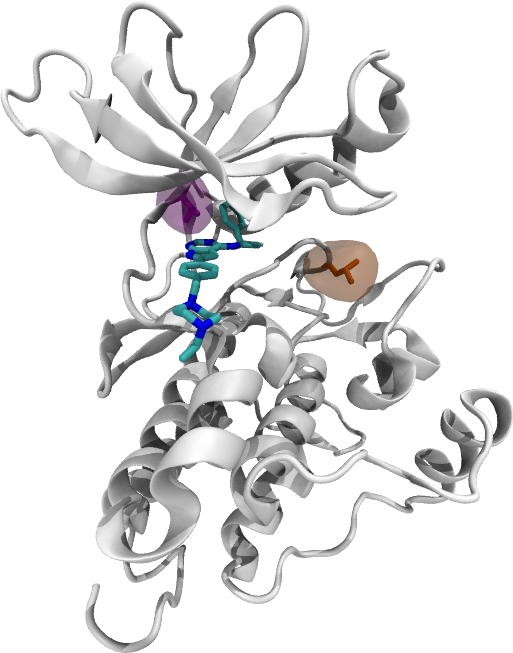
\includegraphics[width=0.60\columnwidth]{FIGURES/egfr.png}
  \caption{Cartoon representation of the EGFR kinase bound to the inhibitor
  AEE788 shown in chemical representation (based on PDB:2J6M). Two residues
  implicated in modulating drug efficacy are highlights; in pink T790 and in
  orange L858. Mutations to either of these residues significantly alter the
  sensitivity to TKIs.}\label{fig:egfr}
\end{figure}


A common target of kinase inhibitors is the epidermal growth factor receptor
(EGFR) which regulates important cellular processes including proliferation,
differentiation and apoptosis. EGFR is frequently over expressed in a range of
cancers, and is associated with disease progression and treatment. Clinical
studies have shown that EGFR mutations confer tumor sensitivity to tyrosine
kinase inhibitors in patients with non-small-cell lung cancer (examples shown
in Fig.~\ref{fig:egfr}) The tyrosine kinase domain of EGFR contains 288
residues, the full simulation system including solvent and the AEE788
inhibitor contains approximately 50 thousand atoms. The well established AMBER
ff99SBildn and GAFF force fields~\cite{Maier2015, Wang2004} were used to
parameterize the system for this work.


% ---------------------------------------------------------------------------
\subsection{Automated binding affinity calculations}

% MD is a well established computational methodology for
% studying the time-evolution and conformational dynamics of a diverse array of
% physicochemical systems at the molecular level, from which a whole host of
% physical and chemical properties can be determined~\cite{Karplus2005}.

The implementation of any physically realistic molecular simulation has
always been an involved and multistage process, often requiring the scientist
to overcome a large manual overhead in the construction, preparation, and
execution protocols needed to complete a set of simulations as well as to
invoke various analysis protocols for determining desired properties
post-production. 

Several tools have been been developed to automate MD workflows for the rapid,
accurate and reproducible computation of binding free energies of small
molecules to their target proteins. For example, BAC~\cite{Sadiq2008} is a
partially automated workflow system which comprises model building (including
incorporation of mutations into patient specific protein models); run of
ensembles of MD simulations, using a range of free energy techniques; and
statistical analysis. In Section 5, we introduce an enhancement of BAC, called
high throughput BAC (HTBAC).

% which utilizes Ensemble Toolkit~\cite{entk}.

% and
% RADICAL-Pilot to create a flexible software framework for runtime execution
% and performance.


% Two protocols of particular importance for XXXX are ESMACS (enhanced
% sampling of molecular dynamics with approximation of continuum
% solvent)\cite{Wan2017brd4} and TIES (thermodynamic integration with
% enhanced sampling) \cite{Bhati2017}. The former is based on variants of the
% molecular mechanics Poisson-Boltzmann surface area (MMPBSA) end-point
% method and the latter the `alchemical' thermodynamic integration (TI)
% approach. In both cases ensembles of MD simulations are employed in order
% to perform averaging and to obtain tight control of error bounds in our
% estimates.

% We have demonstrated the lack of reproducibility of single trajectory
% approaches in both HIV-1 protease and MHC systems, with calculations for
% the same protein-ligand combination, with identical initial structure and
% force field, shown to produce binding affinities varying by up to 12 kcal
% mol $^{-1}$ for small ligands (flexible ligands can vary even more).
% \cite{Wan2015, Sadiq2010, Wright2014} Indeed, our work has revealed how
% completely unreliable single simulation based approaches are. While
% accuracy of force fields could be a source of error, we know from our work
% to date \cite{} that the very large fluctuations in trajectory-based
% calculations account for the lion’s share of the variance (hence also
% uncertainty) of the results. Almost all MMPBSA studies in the literature
% use the so-called 1-trajectory method, in which the energies of
% protein-inhibitor complexes, receptor proteins and ligands are extracted
% from the MD trajectories of the complexes alone. ESMACS protocols can
% additionally use separate ligand and receptor trajectories to account for
% adaptation energies. Previous work has produced results in agreement with
% previously published experimental findings \cite{Sadiq2010, Wan2011,
% Wright2014, Bhati2017, Wan2017brd4, Wan2017trk}, and correctly predicted
% the results of experimental studies performed by colleagues in
% collaboration \cite{Bunney2015}.




% ---------------------------------------------------------------------------
% III - SECTION
% ---------------------------------------------------------------------------
\section{Computational Challenges at Extreme Scale}\label{sec:3}
% \subsection{Computational Challenges}

High-performance computing (HPC) environments were designed to primarily
support the execution of single simulations. Current HPC platforms enable the
strong and weak scaling of single tasks (hitherto mostly simulations), with
limited software and systems support for the concurrent execution of multiple
heterogeneous tasks as part of a single application (or workflow). As the
nature of scientific inquiry and the applications to support that inquiry
evolve, there is a critical need to support the scalable and concurrent
execution of a large number of heterogeneous tasks.

%  each of which is typically smaller than the traditional single simulations
% supported by HPC\@.

% The aggregation of multiple tasks alongside their dependencies are usually
% referred to as ``workflows''.
Sets of tasks with dependencies that determine the order of their execution
are usually referred to as ``workflows''. Often times, the structure of the
task dependencies is simple and adheres to discernible patterns, even though
the individual tasks and their duration are non-trivially distinct. Put
together, it is a challenge to support the scalable execution of workflows on
HPC resources due to the existing software ecosystem and runtime systems
typically found.

Many workflow systems have emerged in response to the aforementioned problem.
Each workflow system has its strengths and unique capability, however each
system typically introduces its problems and challenges. In spite of the many
successes of workflow systems, there is a perceived high barrier-to-entry,
integration overhead and limited flexibility.

Interestingly, many commonly used workflow systems in high-performance and
distributed computing emerged from an era when the software landscape
supporting distributed computing was fragile, missing features and services.
Not surprisingly, initial workflow systems had a monolithic design that
included the end-to-end capabilities needed to execute workflows on
heterogeneous and distributed cyberinfrastructures. Further, these workflow
systems were typically designed by a set of specialists to support large
``big science'' projects such as those carried out at the
LHC~\cite{breskin2009cern} or LIGO~\cite{althouse1992ligo}. The fact that the
same workflow would be used by thousands of scientists over many years
justified, if not amortized, the large overhead of integrating application
workflows with monolithic workflow systems. This influenced the design and
implementation of % workflow system
interfaces and programming models.

However as the nature, number and usage of workflows has evolved so have the
requirements: scale remains important but only when delivered with the
ability to prototype quickly and flexibly. Furthermore, there are also new
performance requirements that arise from the need to support concurrent
execution of heterogeneous tasks. For example, when executing multiple
homogeneous pipelines of heterogeneous tasks, for reasons of efficient
resource utilization there is a need to ensure that the individual pipelines
have similar execution times. The pipeline-to-pipeline fluctuation must be
minimal while also managing the task-to-task runtime fluctuation across
concurrently executing pipelines.

Thus the flexible execution of heterogeneous ensembles\mtnote{Should we
define what an ensemble is?} \jdnote{We defined ensemble in the Methodology
Section: We term this approach ensemble molecular dynamics, “ensemble” here
referring to the set of individual (replica) simulations conducted for the
same physical system.} MD simulations face both system software and
middleware challenges: existing system software that is typically designed to
support the execution of single large simulations on the one hand, and
workflow systems that are designed to support specific use cases or
`locked-in' end-to-end executions. % monolithic workflows.
In the next Section, we discuss the design and implementation of the
RADICAL-Cybertools, a set of software building blocks that can be easily
composed to design, implement and execute domain specific workflows rapidly
and at scale.

% that have the necessary properties.

% \begin{itemize}
% 	\item $N_T$ : Number of tasks
% 	\item ${{n_C}^T}$: Number of cores per task
% 	\item $N_c$ : Number of cores (total)
% 	\item $t_x$ : Time durations of a task
% \end{itemize}



% ---------------------------------------------------------------------------
% IV - SECTION
% ---------------------------------------------------------------------------
\section{Ensemble Toolkit}\label{sec:4}
We have designed RADICAL-Cybertools (RCT) to to be functionally delineated
middleware building blocks and to address some of the challenges in developing
and executing workflows on HPC platforms. HTBAC uses two RCT components,
mainly the Ensemble Toolkit (EnTK) and RADICAL-Pilot (RP).

\mtnote{I do not think HTBAC is a workflow! Should we just say `HTBAC uses
two RCT components\ldots'?} \jhanote{Please review above paragraph.}

EnTK provides the ability to create and execute ensemble- based
workflows/applications with complex coordination and communication but
without the need for explicit resource management. EnTK uses RP as the
runtime system which provides resource management and task execution
capabilities.

RCT eschew the concept of a monolithic workflow systems and uses ``building
blocks''. RCT provide scalable implementations of building blocks in Python
that are used to support dozens of scientific applications on
high-performance and distributed systems~\cite{turilli2016analysis,angius2017converging,treikalis2016repex, balasubramanian2016ensemble,balasubramanian2016extasy}. In this Section we discuss details of RP, EnTK
and HTBAC, understanding how these components have been used to support the
flexible and scalable execution of pipelines.

% ---------------------------------------------------------------------------
\subsection{RADICAL-Pilot}

The scalable execution of applications with large ensembles of tasks is
challenging. Traditionally, two methods are used to execute multiple tasks on
a resource: each task is scheduled as an individual job, or MPI capabilities
are used to execute multiple tasks as part of a single job. The former method
suffers from unpredictable queue time: each task independently awaits in the
resource's queue to be scheduled. The latter method relies on the fault
tolerance of MPI, and is suitable to execute tasks that are homogeneous and
have no interdependencies.

The Pilot abstraction~\cite{turilli2017comprehensive} solves these issues:
The pilot abstraction: (i) uses a placeholder job without any tasks assigned
to it, so as to acquire resources via the local resource management system
(LRMS); and, (ii) decouples the initial resource acquisition from
task-to-resource assignment. Once the pilot (container-job) is scheduled via
the LRMS, it can pull computational tasks for execution. This functionality
allows all the computational tasks to be executed directly on the resources,
without being queued via the LRMS\@. % individually. 
The pilot abstraction thus supports the requirements of task-level
parallelism and high-throughput as needed by science drivers, without
affecting or circumventing the queue policies of HPC resources.

RADICAL-Pilot is an implementation of the pilot abstraction, engineered to
support scalable and efficient launching of heterogeneous tasks across
different platforms.
\subsection{Ensemble Toolkit}

An ensemble-based application is a \textbf{workflow}, i.e., a set of tasks
with dependencies that determine the order of their execution. Subsets of
these tasks can be \textbf{workloads}, i.e., tasks whose dependencies have
been satisfied at a particular time and may be executed concurrently.
Ensemble-based application vary in the type of coupling between tasks, the
frequency and volume of exchange between these tasks, and the executable of
each task. This type of applications requires specific coordination,
orchestration and execution protocols, posing both domain-specific and
engineering challenges.

Ensemble Toolkit (EnTK), the topmost layer of RCT, simplifies the process of
creating and executing ensemble-based applications with complex coordination
and communication requirements. EnTK decouples the description of
ensemble-based applications from their execution by separating three orders
of concern: specification of task and resource requirements; resource
selection and acquisition; and execution management. Domain scientist retain
full control of the implementation of their protocols by programming
ensemble-based applications in terms of what should be executed, when and
where. EnTK automates the process of acquiring the resources needed by those
applications and managing their execution via a runtime system like
RADICAL-Pilot.

% A key objective of EnTK is to provide a solution to the execution of
% ensemble-based applications that is independent of the nature of tasks.

EnTK has been used to develop the ExTASY~\cite{balasubramanian2016extasy}
framework for the execution of MD-based advanced sampling methods. EnTK is
also being utilized to develop ensemble-based applications to execute
workflows in the seismology and climate science. Each use case requires
different workflows, with different types of tasks, executed on specific HPC
resources. EnTK supported the development of a simulation-analysis pattern
for ExTASY, implementing two sampling algorithms for execution of both
multithreaded and MPI tasks on ARCHER, Stampede and Blue Waters HPC machines.
With the same code base, EnTK is being used to develop inversion of
full-waveform, wide-bandwidth data for seismic tomography, and a new
downscaling methodology to quantify the photovoltaic (PV) energy potential in
selected regions of the USA\@.

Currently, EnTK enables the execution of up to \(O(10^4)\) tasks on thousands
of CPU and GPU nodes on the resources of XSEDE, ORNL, NCSA, NWSC and UK NSS,
for a total of eight HPC machines. At this scale, multiple sources of failure
affect execution, producing loss of information and compute time. Thus, fault
tolerance and recovery capabilities are first order concerns of the design of
EnTK\@. As such, EnTK can handle task execution failures, resource-level
failures, and failures of its own subcomponents and subprocesses, including
network connectivity issues.

EnTK exposes four components to the end-user: `Resource Handle', `Pipeline',
`Stage', and `Task'. These enable users to create ensemble-based applications
and specify target resources for their execution. Internally the `Application
Manager' and `Execution Manager' components enable the acquisition of
resources and the management of application execution (see
\textbf{Figure~\ref{fig:entk_arch}}, right schematic of left panel).

\begin{figure}[!htbp]
  \centering
  %\begin{minipage}[b]{0.6\textwidth}
  \begin{minipage}[b]{0.55\textwidth}
  \centering
  % 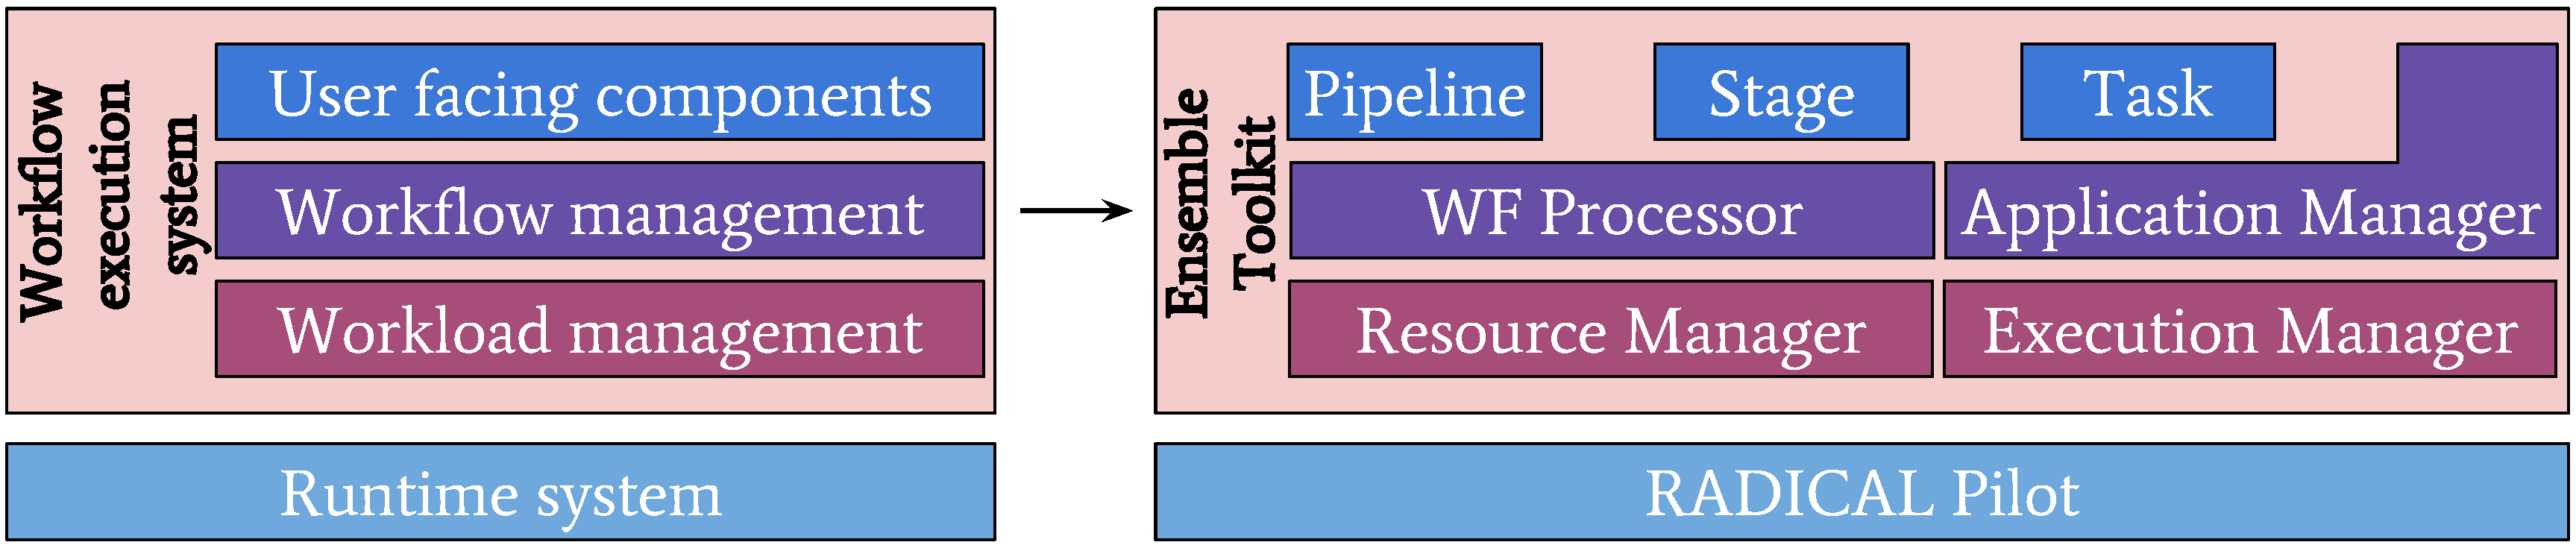
\includegraphics[width=\textwidth, height=35mm]{FIGURES/entk_overview.pdf}
  % 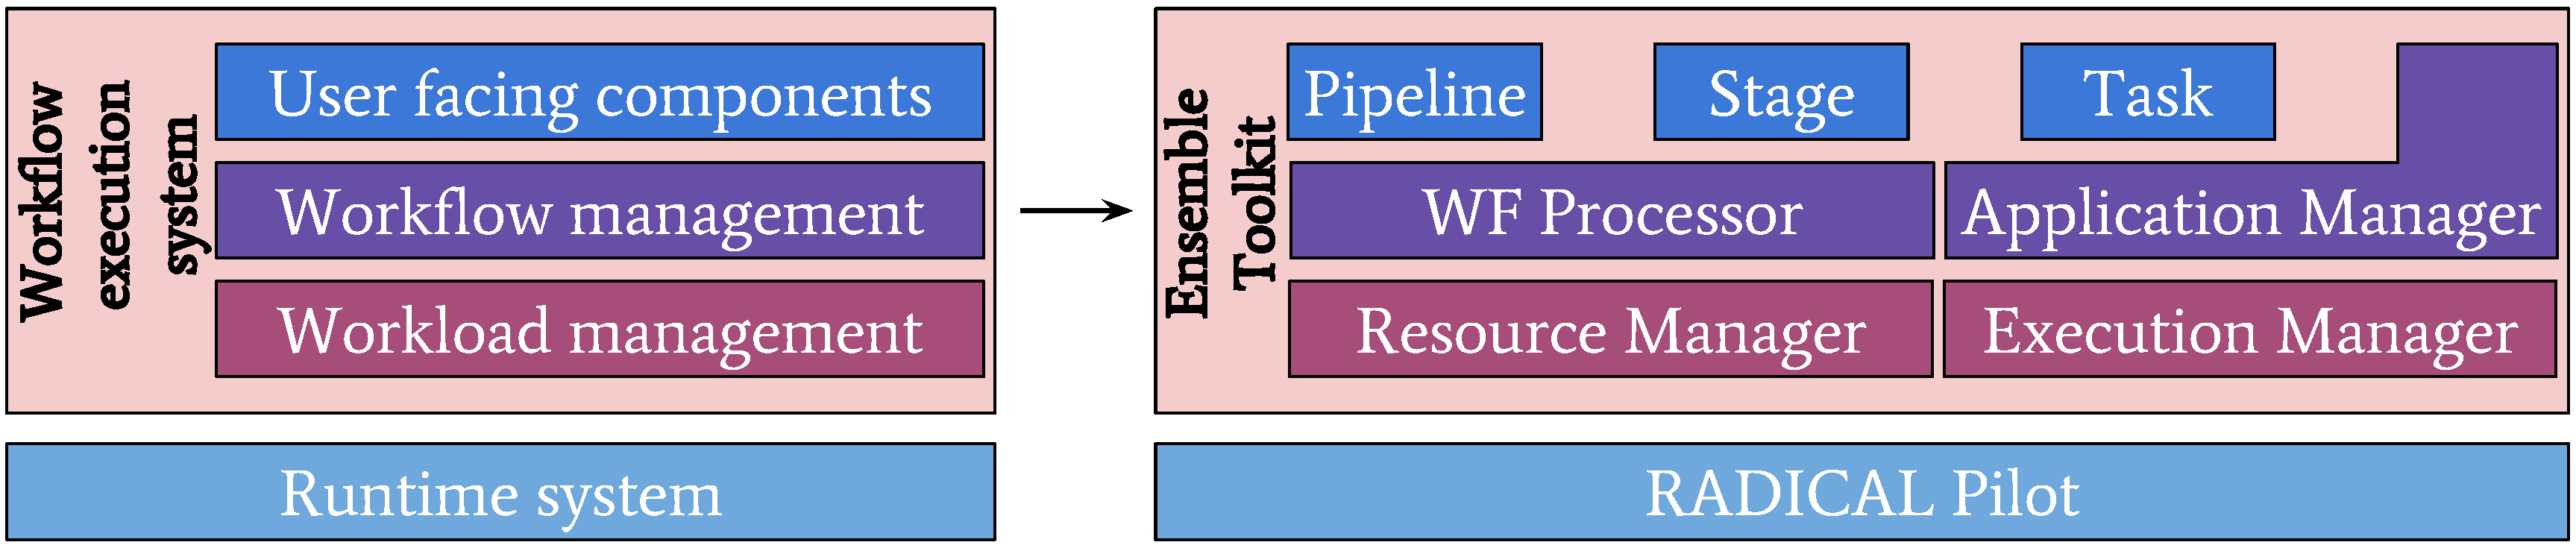
\includegraphics[width=\textwidth, height=40mm]{FIGURES/entk_overview.pdf}
  \end{minipage}
  % \begin{minipage}[b]{0.39\textwidth}
  \begin{minipage}[b]{0.44\textwidth}
  \centering
  % \includegraphics[width=\textwidth, height=35mm]{FIGURES/md_general.pdf}
  % \includegraphics[width=\textwidth, height=40mm]{FIGURES/md_general.pdf}
  \end{minipage}
  \caption{\textbf{Left:} Ensemble Toolkit overview, showing how the abstract
  workflow execution system is mapped to specific components exposed to the
  users and components internal to the toolkit \textbf{Right:} General MD
  workflow overview that broadly describes the science methods to study the
  physical systems}\label{fig:entk_arch}
\end{figure}

The \textbf{Resource Handle} component is used to describe the set of
resources to be utilized. This includes properties like walltime, number of
nodes, or credentials of resources. The \textbf{Task} component is used to
indicate an executable alongside its input/output data and the requirements
for its executing environment. The \textbf{Stage} component is used to group
tasks that have the same dependencies and can be executed concurrently, while
the \textbf{Pipeline} component is used to describe a sequence of stages,
i.e., stages that need to be executed sequentially, not concurrently.

EnTK enables users to program ensemble-based applications directly in Python,
without requires a domain-specific language. The use of the Task, Stage, and
Pipeline components avoids the need to express explicitly relationship among
tasks. These relationships are insured by design, depending on the
partitioning of the set of tasks into stages and then pipelines. Further,
EnTK enables an explicit definition of pre and post conditions on the
execution of tasks, stages, and pipelines, enabling a fine graned adaptivity,
both a local and global level. Conveniently, this does not require the
codification of a DAG, a process that imposes a rigid repreentation model on
the domain scientists.

Once the workflow of an ensemble-based application is completely described,
one or more pipelines are submitted to the \textbf{Application Manager}
module for execution. The Application Manager sets up a messaging
infrastructure to enable fault tolerance and then processes each pipeline,
identifying tasks which have their dependencies satisfied and can be executed
concurrently. These tasks are then handed over to the \textbf{Execution
Manager} that binds tasks to resources on the base of a set of
heuristic-based decisions called `execution strategy'. The Execution Manager
then uses the underlying runtime system, RADICAL-Pilot, to execute the tasks
on the specific target resource.

EnTK is implemented as a multiprocess application. The number of processes
can be tuned to match the throughput requirements of ensemble-based
applications and the capabilities of diverse target resources. All but the
master process of the toolkit are stateless, enabling process-level fault
tolerance. Upon failure of one or more stateless process, application tasks
can be assigned to existing or newly created processes without blocking the
overall execution. Upon failure of the master process, execution can be
restarted without loosing data about tasks that have been already executed.

% Scalability results from an early version of EnTK are provided in
% \textbf{Figure~\ref{fig:entk_perf}}. The number of simulations and the
% total number of cores used are described on the abscissa with each
% simulation using one core; the analysis task which uses one core). Thus,
% the simulation execution time corresponds to the time taken by all the
% simulations to complete.  The analysis execution time corresponds to the
% time taken to analyze the output of all the simulations. Notice how both
% strong and weak scaling up to $O(10^3)$ are linear. Although performance
% numbers are for Stampede (TACC), it is reasonable to expect the weak and
% strong scaling of EnTK to hold firm on Titan as well. The task launching
% and coordination system use the same underlying runtime system --
% RADICAL-Pilot, which has been tested for strong and weak scalability on
% Titan~\cite{angius2017converging} up to $O(10^3)$ tasks. Currently, EnTK
% and RADICAL-Pilot support the execution of ensemble-based applications up
% to $O(10^4)$ tasks. At the next release, planned for Sep 2017, EnTK will
% support $>$ $O(10^4)$ tasks. During the lifetime of this INCITE project
% EnTK is being re-designed, implemented and optimized to reach
% $O(10^5-10^6)$ concurrent tasks, independent of the size and type of task.

\begin{figure}[!htbp]
\centering
\begin{minipage}[b]{.49\textwidth}
  \centering
  %  \includegraphics[width=\textwidth]{FIGURES/entk_perf_strong.pdf}
  %  \caption{Strong scaling behavior of Ensemble Toolkit. The
  %  total workload is kept constant at 1024 simulations and the amount of
  %  resources used are varied from 64 to 1024. We observe close to linear
  %  drop in the simulation execution time as the amount of resources are
  %  doubled}
\end{minipage}
\begin{minipage}[b]{.49\textwidth}
    \centering
  %  \includegraphics[width=\textwidth]{FIGURES/entk_perf_weak.pdf}
  %  \caption{Weak scaling behavior of Ensemble Toolkit. The size of the
  %  workload is varied in proportion with the amount of resources such that
  %  all tasks are concurrently executed at all times. We observe similar
  %  simulation execution times at all configurations.}
\end{minipage}
\caption{\textbf{Left:} Strong scaling of EnTK. The total workload is kept
        constant at 1024 simulations and the resources used are varied from
        64 to 1024 cores. We observe essentially linear drop in the
        simulation execution time. \textbf{Right:} Weak scaling of EnTK. The
        size of the workload is varied in proportion with the amount of
        resources such that all tasks are concurrently executed at all times.
        We observe similar simulation execution times at all
        configurations.}\label{fig:entk_perf}
\end{figure}



% ---------------------------------------------------------------------------
% V - SECTION
% ---------------------------------------------------------------------------
\section{High Throughput Binding Affinity Calculator}\label{sec:htbac}

HTBAC is a workflow system that uses RCT to implement ESMACS, and similar
protocols such as TIES\@. These protocols consist of pipelines with stages
comprised of heterogeneous tasks. For example, equilibration and production,
followed by post processing steps. The different protocols supported by HTBAC
differ in the details of the pipelines, stages and
synchronization~\cite{Bhati2017}.

\mtnote{I am not able to understand this paragraph so I am not able to propose
an alternative. I believe it should be rewritten.}\jhanote{OK?}

RADICAL-Cybertools provides advanced resource management capabilities and,
thereby delivers the necessary high- throughput capabilities required.HTBAC is
integrated with the EnTK component of RCT. EnTK provides a common API,
execution and programming model, thus allowing HTBAC to express the workflows
associated with different protocols uniformly, and thus minimize development
effort and complexity.

The Ensemble Toolkit API exposes four components (\textbf{Resource Handle},
\textbf{Pipeline}, \textbf{Stage}, and \textbf{Task}) to express the
application logic of HTBAC\@. We describe these components for the ESMACS
protocol\@. The concept of an ensemble in the ESMACS protocol maps directly to 
a set of pipelines in EnTK, where each pipeline contains functions that operate 
on a given replica. EnTK interprets these replicas as independent pipelines. 
Each pipeline consists of multiple stages representing a well-defined execution 
order; each stage can contain heterogeneous workloads. Although each stage of a 
pipeline depends on its predecessor, the pipelines execute independently of each 
other. The pattern within pipelines are identical and describes an ensemble of replica
simulations as shown in Fig~\ref{figure:ESMACS-pipelines}.

\jhanote{DWW, should we not use replica?}
\dwwnote{Shantenu, I have tried to make a consistent mapping above 
         and in the figure caption. Does this work for you?}\jhanote{cool!}

\begin{figure}
\centering
  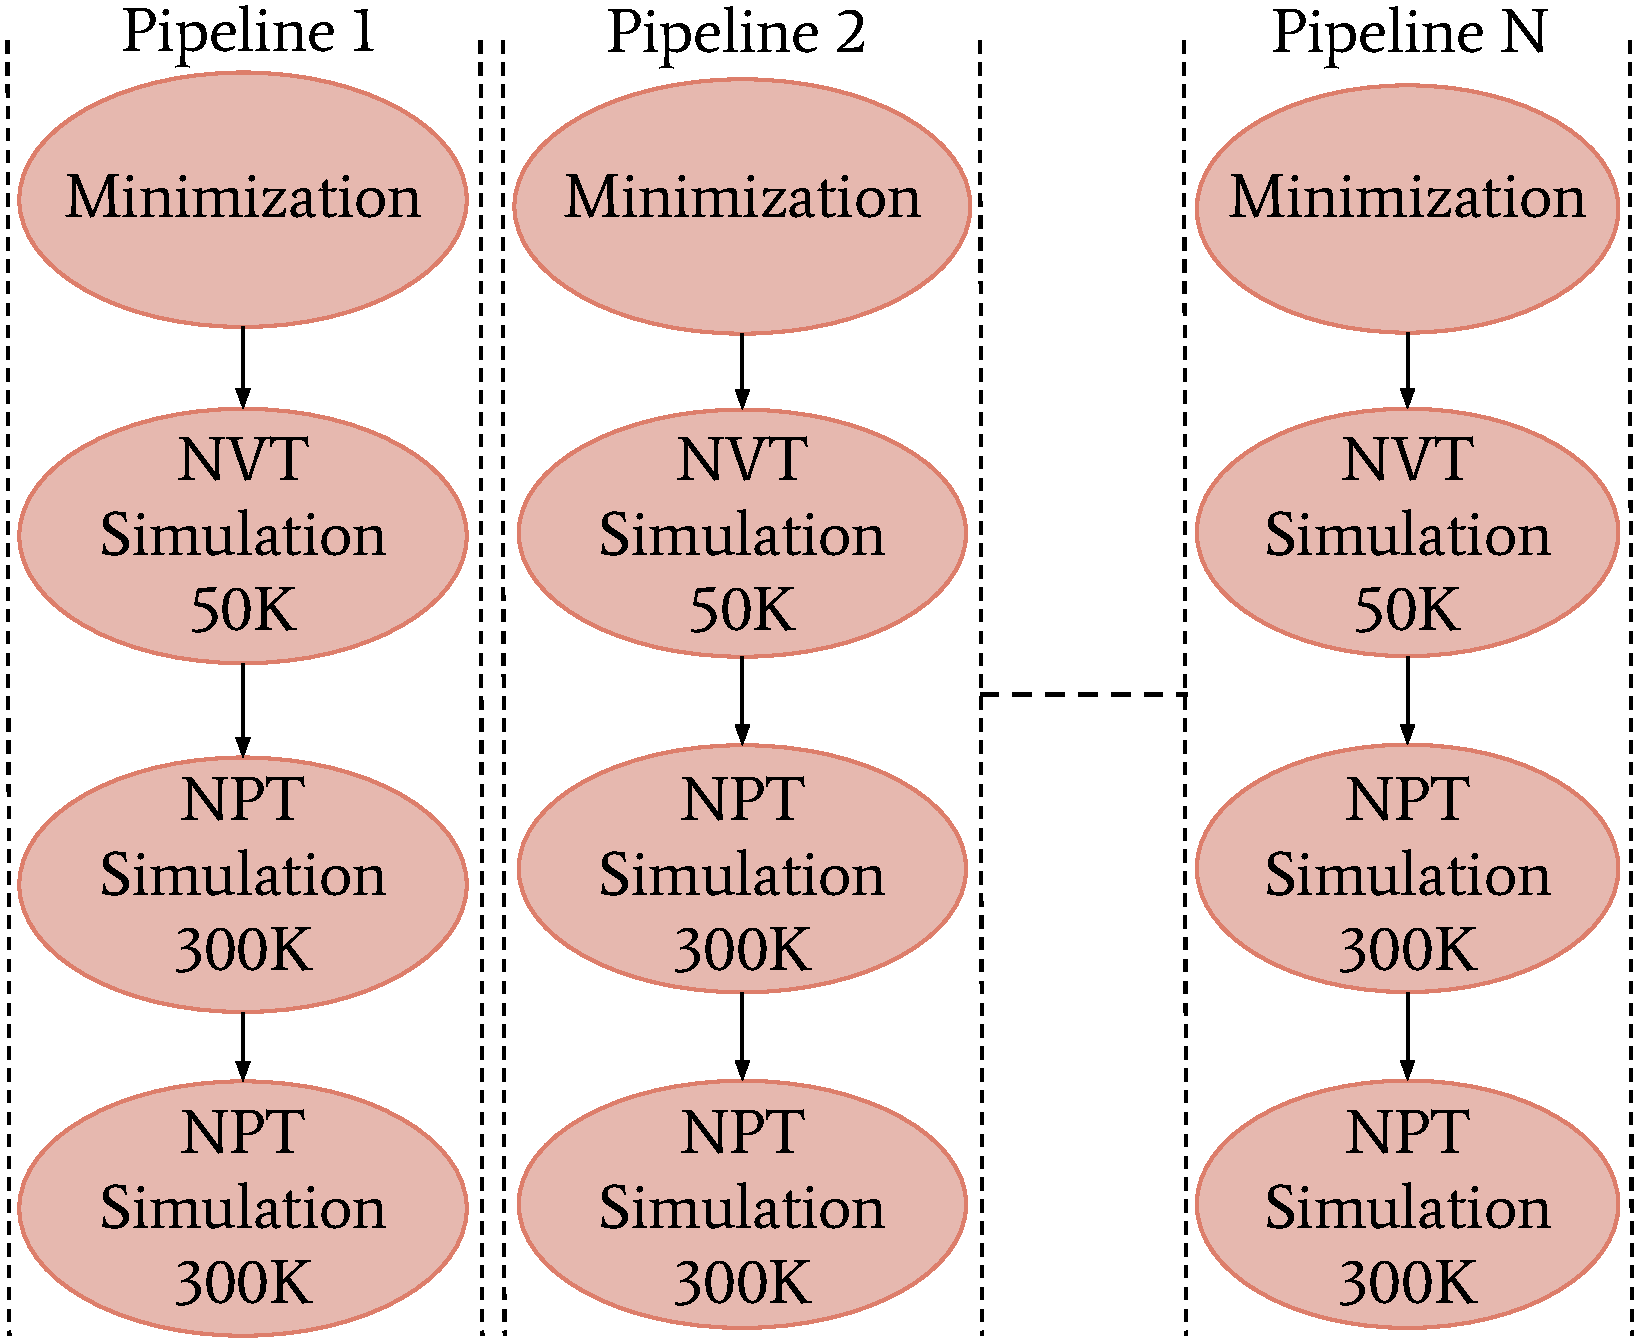
\includegraphics[width=0.5\textwidth]{FIGURES/HT-BAC_NAMD_pipelines_control_flow_only.pdf}
  \caption{ESMACS protocol indicating how an N replica ensemble is implemented in HTBAC.
  Each replica is mapped to a single EnTK pipeline. 
  Each pipeline is equivalent and represents a set of simulations which are captured as stages by
  EnTK.}\label{figure:ESMACS-pipelines}
\end{figure}

%\begin{itemize}
%	\item 1) Untar configuration files
%	\item 2) Preprep
%	\item 3) Minimize with decreasing restraints
%	\item 4) Equilibration: NVT simulation at 50K, with restraints
%	\item 5) Equilibration: NPT simulation at 300K, with decreasing
%	restraints
%	\item 6) Equlibratin: NPT at 300k, no constraints
%	\item 7) Tarball output files 
%\end{itemize}

Each stage is composed of a single unique task which is described by a set of
attributes that define the workload parameters such as the location of input
files, the number of simulations and the MD engine(s) to launch simulations.
The ESMACS protocol defines 7 stages, in which the preliminary and last
stages perform staging the input/output data. The middle stages indicate
simulation tasks as shown in Fig~\ref{figure:ESMACS-pipelines}. The task is
appended to a stage and stages are appended to a pipeline to maintain
temporal order. The workflow relies on a resource configuration which
consists of the details required to use a resource where the application will
be executed including runtime, queue, and account details. We capture the
integration of the application (ESMACS protocol) and how it interfaces with
EnTK in Fig~\ref{figure:ht-bac_rp}.

We define the client resource in Fig~\ref{figure:ht-bac_rp} as the workload
system---HTBAC which describes a series of replicas with ordered functions as
a pipelines with stages and tasks. EnTK interprets these pipelines as a
functional set of tasks and generates the pilot description that contains the
resource configuration of how to run the HTBAC workload. For the ESMACS
protocol running on Blue Waters we define the runtime system, queue, and the
pilot size. Once RADICAL-Pilot receives this new workload it generates a
pilot that submits placeholders to the queue. Once the pilot is activated,
the RP-Agent submits the tasks in the form of compute units to the
placeholders to begin execution.

\begin{figure}
\centering
  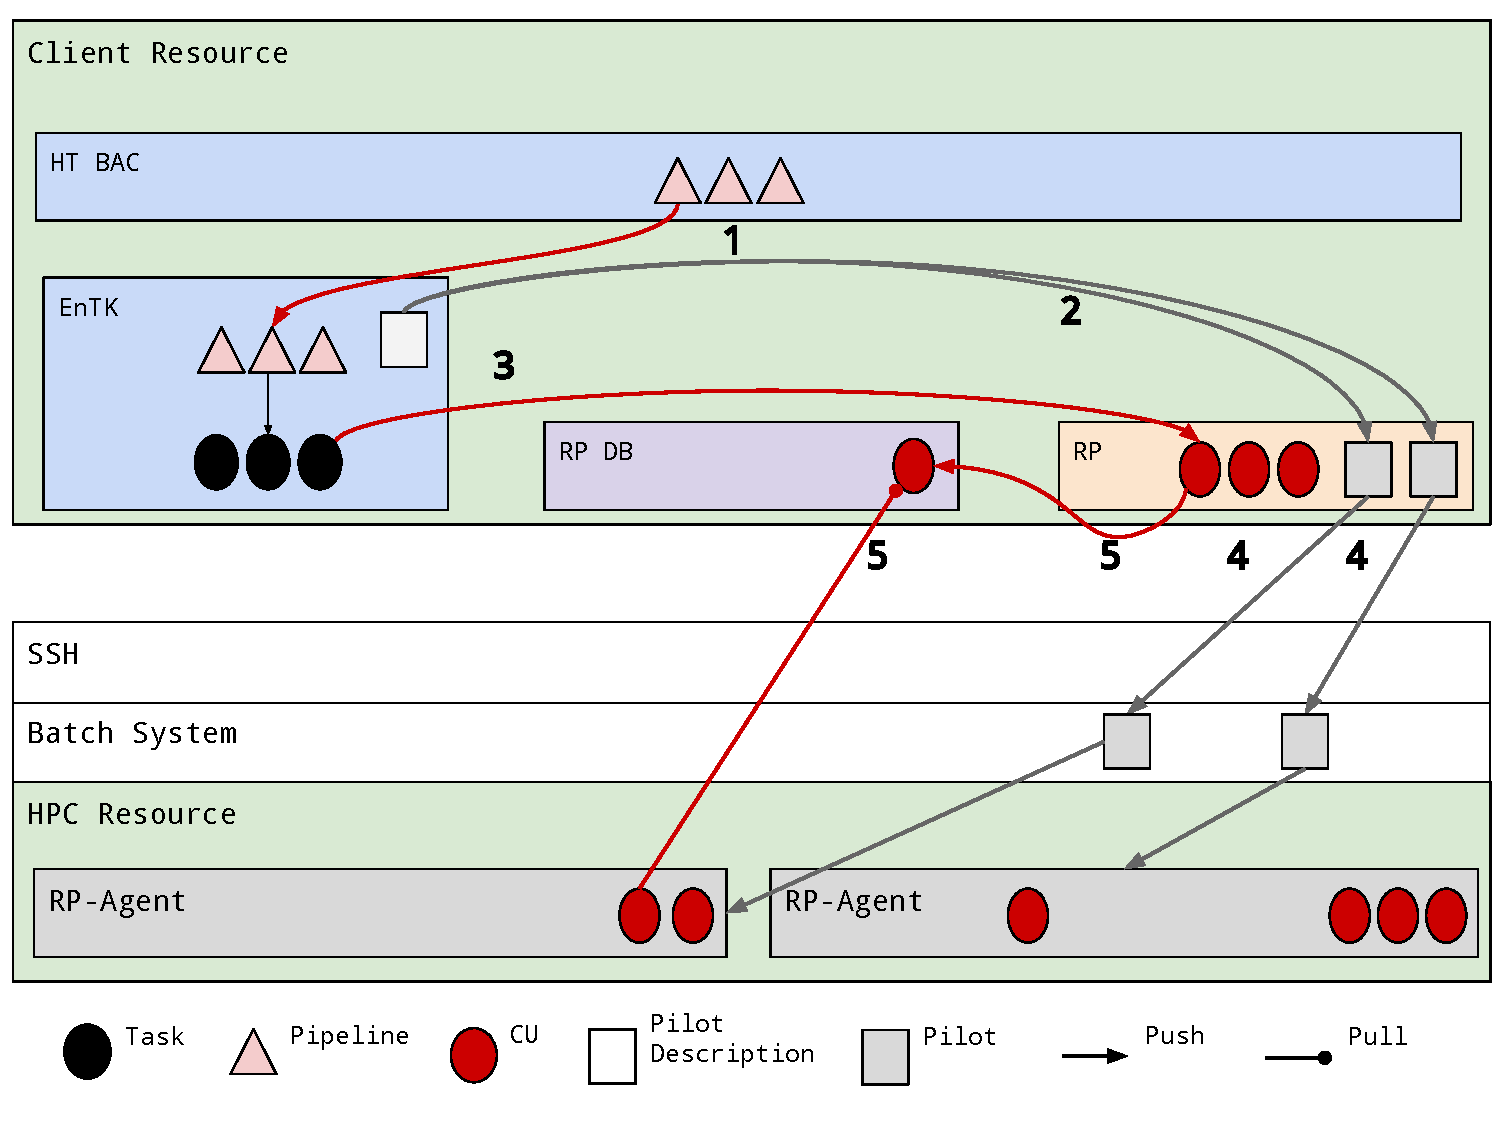
\includegraphics[width=0.5\textwidth]{FIGURES/ht-bac-rp_integration.pdf}
  \caption{\bf Integration between HTBAC workflow and EnTK\@. Numbers
  indicate the temporal sequence of execution. RADICAL-Pilot (RP) database
  (DB) can be deployed on any host reachable from the
  resources.\dwwnote{I think CU needs to be defined here}}\label{figure:ht-bac_rp}
\end{figure}



%\begin{figure}[ht]
%\centering
%  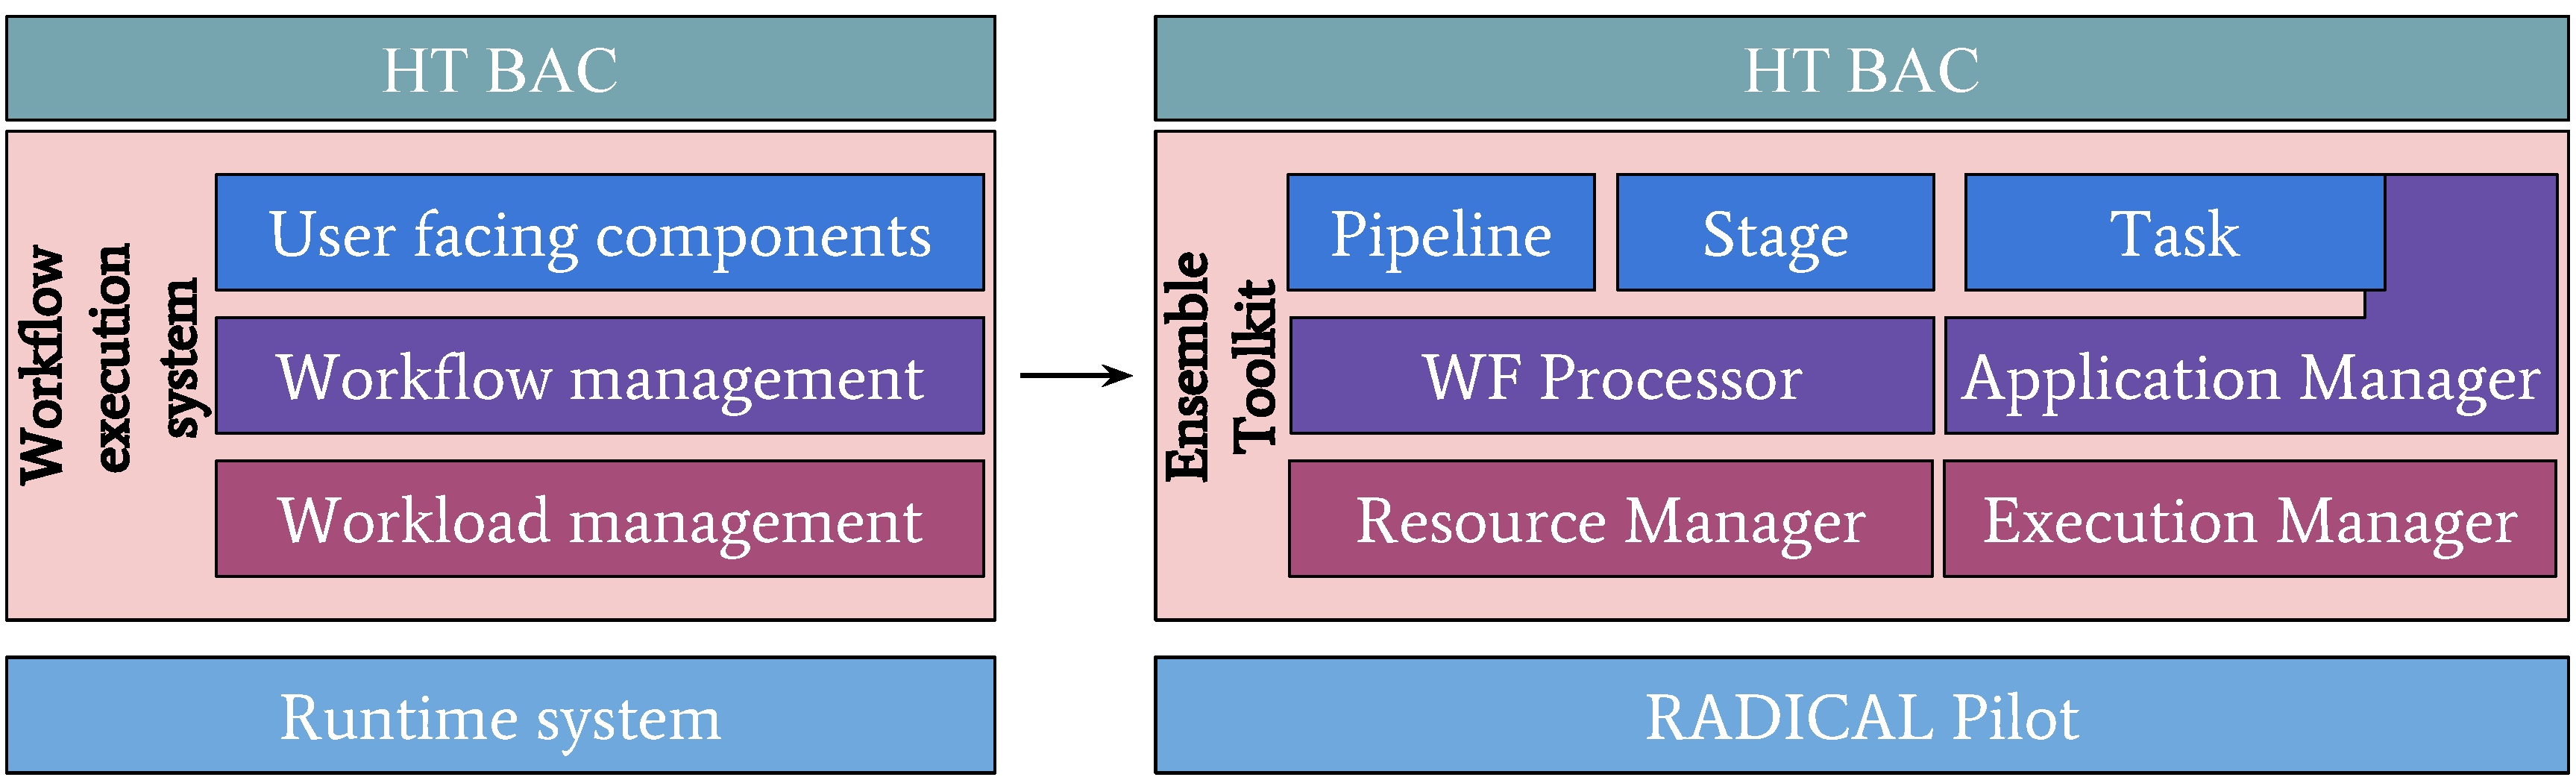
\includegraphics[width=0.5\textwidth]{FIGURES/entk_htbac_integration.pdf}
 % \caption{\bf Integration between HT-BAC workflow system and EnTK that shows resource/application managers.}
   %\label{figure:ht-bac_entk}
%\end{figure}




% ---------------------------------------------------------------------------
% VI - SECTION
% ---------------------------------------------------------------------------
\section{HTBAC Experiments}\label{sec:6}
% \subsection{Characterization of Performance}

Before embarking in a computational campaign that will consume 150M core
hours on the NCSA Blue Waters machine, we study the scalability of the ESMACS
protocol to determine optimal workflow sizing and resource utilization. The
goal is twofold: (1) understanding the invariance of HTBAC execution time
over the number of workflow pipelines executed; and (2) studying how
EnTK---the RCT tool responsible for coordinating the distributed execution of
the protocol---scales its performance in relation to the size of HTBAC
workflow.

% ---------------------------------------------------------------------------
\subsubsection{Experiment Design}\label{ssec:exp_design}

We designed two experiments to measure HTBAC and EnTK weak scalability when
executing an increasing number of concurrent pipelines. According to the use
case described in Section~\ref{sec:htbac}, each pipeline consists of seven
stages, each stage with a single task. EnTK manages the queuing of the tasks
in accordance with the order and concurrency mandated by stages and
pipelines: For each pipeline, each stage is executed sequentially while
pipelines are executed concurrently.

%\mtnote{PLease note: I converted the following paragraph eliminating
%references to RP\@. This is consistent with out decision of not showing RP
%overheads. The paragraph can be reused if we change our mind. `` We validate
%the performance of EnTK % the runtime system, RADICAL-Pilot, using weak
%scalability to to show % demonstrate that EnTK % RP can schedule tasks
%concurrently, provided that sufficient resources
%areavailable.''}\jhanote{+1}

Experiment 1 measures the baseline behavior of EnTK with the HTBAC workflow
and a null workload (\textmd{/bin/sleep 0}). The goal is to isolate the
overheads of EnTK from the specifics of: (1) the executables of the HTBAC
workflow; (2) the runtime used to execute the workflow on the HPC resources;
and (3) the overheads of the resources. The null workload does not require
data staging, I/O on both memory and disk, or communication over network.

Experiment 2 replicates the design of Experiment 1 but it executes the HTBAC
workflow with the use-case workload. The comparison between the two
experiments enables performance analysis of EnTK to understand whether and
how the size of the executed workflow affects its overheads. Further,
Experiment 2 shows also whether HTBAC is sensitive to the number of
concurrent pipelines executed.

% In order to show % demonstrate 
% that % RP 
% EnTK is invariant to the type of workload, we run two types of experiments:
% We ran the HTBAC workflow with null workload in which each task did no work
% (/bin/sleep 0), the actual simulation workload. 

Both experiments measure the weak scalability of HTBAC and EnTK\@. This means
that the ratio between the number of pipelines and cores is kept constant by
design. While an investigation of strong scalability would contribute to a
better understanding of the behavior of both HTBAC and EnTK, it is of limited
interest for the current use case. The driving goal of HTBAC is to increase
throughput by a means of concurrency, not in the number of sequential execution per
core. This is one of the reasons because our project targets large HPC
machines instead of so-called HTC infrastructures.

% We illustrate the high throughput capabilities of the HTBAC workflow using
% ESMACS protocol by examining scalability in the number of pipelines and
% characterizing the performance of the workload. We show that the
% scalability we measure of the workflow is unrelated to the scalability of
% EnTK\@.

% ---------------------------------------------------------------------------
\subsubsection{Experiment Setup}\label{ssec:exp_setup}

We perform both Experiment 1 and 2 % scalability experiments 
on the Blue Waters HPC cluster---a 13.3 petaFLOPS Cray at NCSA and University
of Illinois, with 32 Interlago cores/50 GB RAM per node, Cray Gemini, Lustre
shared file system. Currently, we exclusively use CPUs on Blue Waters as GPUs
are not required by our use case. RCTs support the use of both type of
architectures and we previously benchmarked the use of GPUs for later
evaluation.

% We characterize the weak scalability of the ESMACS protocol using Ensemble
% Toolkit running exclusively on Blue Waters CPUs.

We perform our experiments from a virtual machine hosted in Europe. This
helps to simulate the conditions in which the experimental campaign will be
performed by the research group at UCL\@. This is relevant because, as most
HPC resources, Blue Waters does not allow for executing applications on the
login node of the cluster. To this end, RCTs support \textmd{gsissh} for X509
authentication and authorization.

Table~\ref{tab:exp} shows the setup for Experiment 1 and 2. Currently, the
ESMACS protocol is executed with up to 25 concurrent pipelines. This number
is suboptimal as pipelines are independent and therefore their concurrent
execution does not entail communication overhead. Further, the system
simulated can benefit from concurrency because potential HTBAC users may wish
to extend their protocols beyond the current scale of ESMACS\@. Consistently,
our experiments push the boundaries of current scale by executing 8, 16, 32,
64 and 128 concurrent pipelines.

\begin{table*}[t]
\centering
\caption{\bf Experiment 1 executes the 7 stages of the ESMACS protocol with
a null workload; Experiment 2 uses the actual workload of the ESMACS
protocol. ESMACS protocol with NAMD and supporting workload: (1) Untar
configuration files; (2) Preprep; (3) Minimize with decreasing restraints;
(4) Equilibration: NVT simulation at 50K, with restraints; (5) Equilibration:
NPT simulation at 300K, with decreasing restraints; (6) Equilibration: NPT at
300k, no constraints; (7) Tarball output files.}\label{tab:exp}
\begin{tabular}{lrrrrr}
\hline
%\multicolumn{1}{l|}{Experiment ID \& Description} & \multicolumn{1}{l|}{Trials} & \multicolumn{1}{l|}{Pipelines} & \multicolumn{1}{l}{Stages} & \multicolumn{1}{l|}{Tasks} & \multicolumn{1}{l}{Total Number of Cores} \\ \hline
\multicolumn{1}{l}{\textbf{Experiment ID \& Description}} & \multicolumn{1}{r}{\textbf{Trials}} & \multicolumn{1}{c}{\textbf{Pipelines}} & \multicolumn{1}{r}{\textbf{Stages}} & \multicolumn{1}{r}{\textbf{Tasks}} & \multicolumn{1}{r}{\textbf{Total Number of Cores}} \\ 
\hline
1 (Null workload)                                           & 2                           & 8, 16, 32, 64, 128             & 7                           & 7                          & 64, 128, 256, 512, 1024                    \\ %\hline
2 (NAMD and Supporting Workload)                                       & 2                           & 8, 16, 32, 64, 128             & 7                           & 7                          & 64, 128, 256, 512, 1024                    \\ \hline
\end{tabular}
\end{table*}


% requires The amount of replicas required by has an upper-bound of 25
% replicas yet we extend the number replicas to 128 in order to show higher
% scalability with a greater degree of confidence for the potential HTBAC
% user.

EnTK uses RADICAL-Pilot to acquire resources via a single pilot. The size of
the pilot is contingent upon characterization of performance, in this case,
weak scalability. Accordingly, we use the same number of cores in a pilot as
those required by the workload.% The number of cores is varied 
We use between 64 and 1024 cores in both Experiment 1 and 2, and we always
keep the number of simulations equal to the number of cores. % at all times. 
We use either 1 or 8 cores per task % replica, 
depending on the task requirements.

% \mtnote{The following needs discussion: ``The size of the workload is
% varied in proportion to the amount of resources such that all tasks are
% concurrently executed at all times.'' I believe this is not necessary true:
% we do not execute all the tasks concurrently all the time but we always get
% enough cores to run at least one task from each concurrent pipeline.
% Alternatively, at every point in time, there are enough cores so that
% pipelines do not compete for the same core.}\jhanote{I agree we do not run
% all the tasks concurrently.}

% \mtnote{I would represent the following with a table. Please feel free to
% change it back if you disagree. ``For example, in the ESMACS protocol, the
% simulation task specifies 8 cores per pipeline, therefore the pilot size is
% defined as 8 \(\times \) number of pipelines. We vary the number of
% pipelines to characterize weak scaling performance where the tasks are
% scheduled concurrently.''}

% \mtnote{The following should probably moved to the next subsection, when
% discussing the results of the experiments: ``For each of these
% configurations, the simulation execution time is observed to be
% constant.''}
% \jhanote{yes}

All the experiments use Ensemble Toolkit version 0.4.7 and RADICAL-Pilot
version 0.42. In the MD workload of the HTBAC workflow, the simulation tasks
are executed using NAMD-MPI\@. The equilibration % stages 
tasks of stage 4 and 6 are assigned 5000 timesteps while the task of stage 5
requires 55000 timesteps. We ran both the null and MD workload for two trials
at each pipeline configurations.

% ---------------------------------------------------------------------------
\subsubsection{Results}\label{ssec:exp_results}

First we characterize the overhead of RADICAL-Pilot (RP) and EnTK in the 
null workload, where we isolate the % any 
overhead introduced by the two % application
systems (Figure~\ref{fig:exp1}). We see a (slightly) superliner
increase of EnTK overhead, between 0.1 and 1.8 seconds. This overhead depends
on the number of tasks that need to be translated in-memory from a Python
object to a compute unit (CU) description. As such, it is expected to grow
proportionally to the number of tasks, barring some competition of resources
on a shared workstation like the one used for our experiments.

\begin{figure}
  \centering
  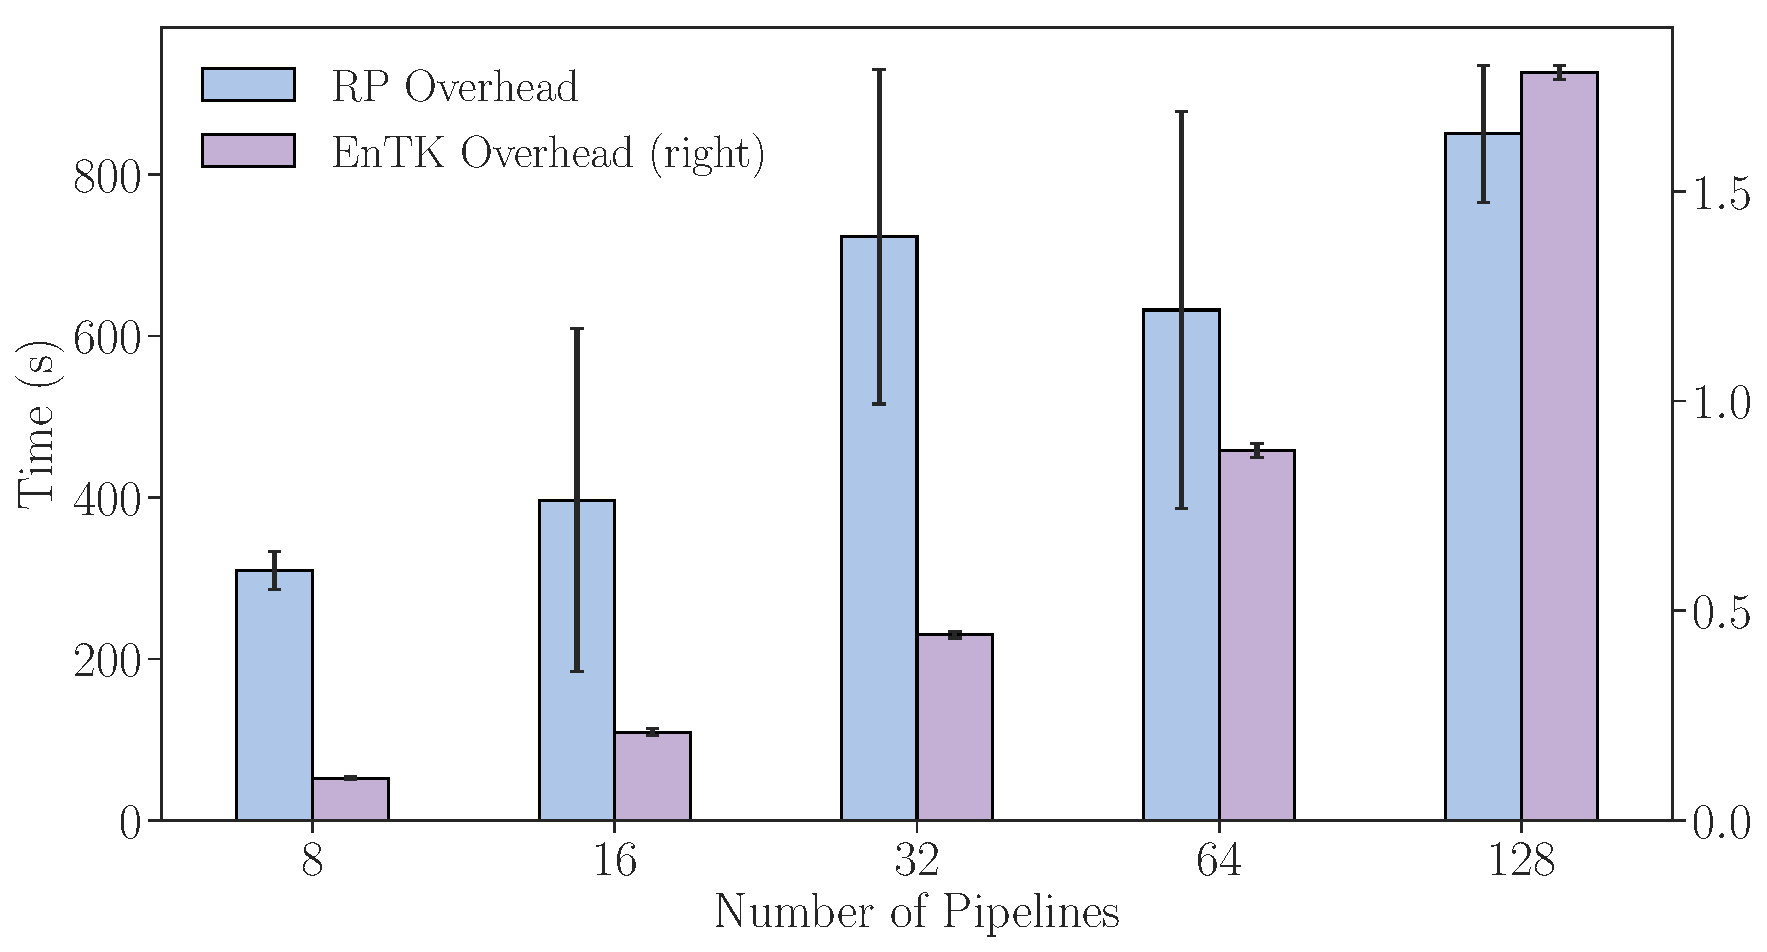
\includegraphics[width=\columnwidth]{FIGURES/null_workload_overheads.pdf}
  \caption{Overheads of Ensemble Toolkit (EnTK) and RADICAL-Pilot (RP) when
           executing HTBAC using a null workload. We plot the baseline
           EnTK/RP overheads without the application workload across two
           trials per pipeline configuration.}\label{fig:exp1}
\end{figure}

% Weak scaling of HTBAC using null workload. We observe similar behavior at
% each configuration in the simulation execution time showing that the EnTK
% is invariant to the workload and a steady increase in the RP overhead due
% to the increase in the number of stages

RP overhead is also, on average, superlinear but with a much greater
variance. This variance is due to mainly two factors: Network latency and
filesystem latency on the HPC resource. EnTK submits CU descriptions to the
MongoDB used by RP, and RP pilot pulls these descriptions from the same
database. As described in Section~\ref{ssec:exp_setup}, this pull operation
occurs between Germany and USA, introducing varying amount of latency.
Further, RP pilot writes and reads the CU descriptions multiple time from to
and from the shared filesystem of the HPC machine. Together, these two
factors introduce delays in the scheduling of the CUs.

% We see a steady superlinear increase in the RP and EnTK overheads as we
% grow the number of pipelines. Note that the RP overhead also captures the
% overhead introduced by the Blue Waters file system, network communication,
% time to stage the units and communication to the database.

As we introduce the use-case NAMD and supporting workload
(Figure~\ref{fig:exp1}), we show that the RP overhead becomes
% insignificant 
on average less than 10\% of the average total execution time (TTX), defined 
as \(TTX = TTC - T_q\) where \(TTC\) is time-to-completion and \(T_q\)
% where we measure TTX as 
is time spent queuing on the HPC machine. We notice the TTX scales weakly
across pipelines of different size and that, when accounting for variance, RP
overheads also shows weak scaling behavior. As expected, EnTK overhead
remains superlinear and comparable to the one measured in Experiment 1. This
is because in both experiments EnTK overhead depends on the number of tasks
translated to CU descriptions.

\begin{figure}
  \centering
  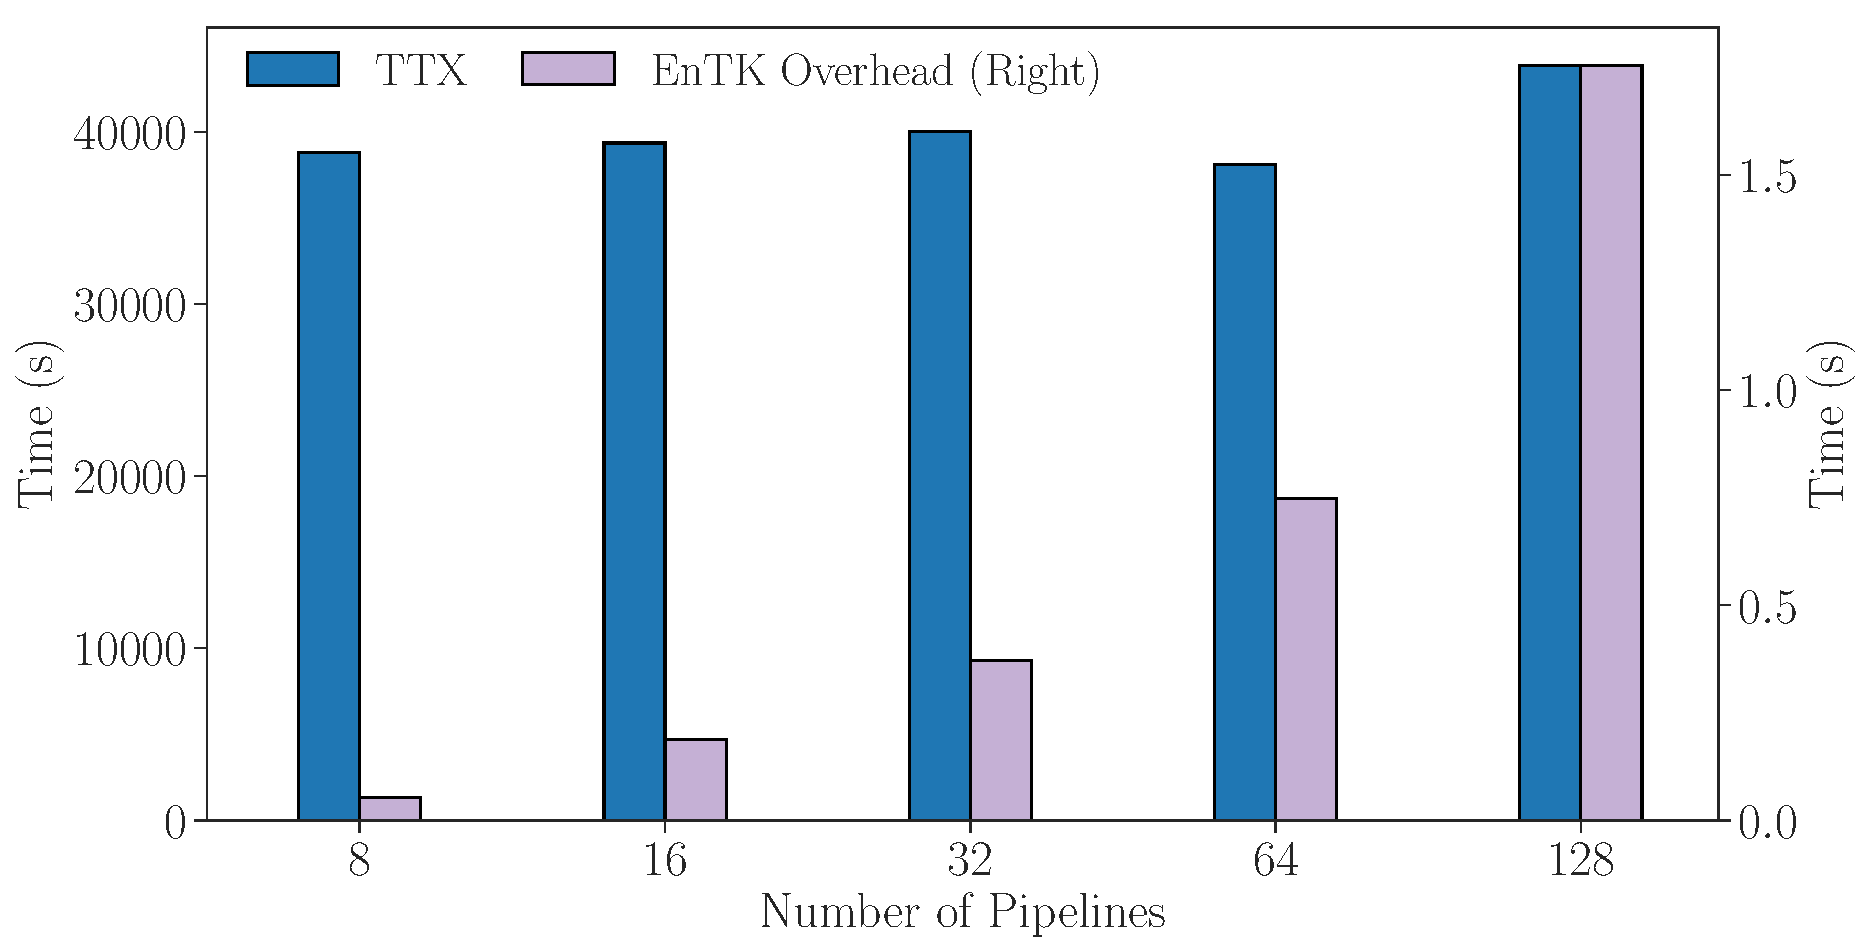
\includegraphics[width=\columnwidth]{FIGURES/namd_workload_overheads.pdf}
  \caption{Introducing the use-case NAMD and supporting workload, we observe
  similar EnTK/RP overhead behavior as with the null workload with higher
  values as the number of pipelines increases. Across pipeline
  configurations, TTX and RP overheads (accounting for the error bars) show % a correct trend in 
  weak scaling performance.}\label{fig:exp2}
\end{figure}

% Weak scaling of HTBAC using use-case payload. We observe higher
% time-to-completions for each  than the null workload yet similar
% performance across pipelines indicating optimal weak scaling
% characterization

Experiments 1 and 2 show how the overheads of both EnTK and RP tend to be
invariant across type of workload executed. Their scaling behavior and, to
some approximation, their absolute values are comparable between
Figure~\ref{fig:exp1} and~\ref{fig:exp2}. This is relevant because it shows
that the systems used to coordinate and execute the ESMACS protocol add a
constant and comparatively not relevant overhead to the execution of NAMD\@.

% In both payloads, the RP and EnTK overheads showed an invariance to
% the type of payload.

% Moreover we validate the concurrency in the execution of tasks based on the
% performance of weak scaling in the use-case workload where the execution
% time (TTX) behaves similarly as the pipeline configuration is increased.

% The RP overhead demonstrates the core overhead which is the
% time-to-completion (TTC) as measured by RADICAL Pilot as well as the Blue
% Waters file system overhead, network communication, time to stage the
% units, and the latency of communication to the database.

% For the NAMD workload, we show weak scaling results for the overheads and
% the simulation execution time which corresponds to the time taken by all
% the simulations to complete.

% The fluctuation of the simulation execution times can be attributed to
% run-time system fluctuations within the workload including stragglers at
% higher pipeline and pipeline-to-pipeline fluctuations. In order to examine
% the fluctuations within stages we correlate the overhead for each pipeline
% at the longest simulation duration in order to reconcile any fluctuations
% induced by NAMD\@. We calculate time-to-execution (Tx) of the largest
% pipeline size and compare the longest MD run within each pipeline. The NAMD
% logs indicate a mean and variance as\ldots

% \begin{figure}[!htbp]
%   \centering
%   %\begin{minipage}[b]{0.6\textwidth}
%   \begin{minipage}[b]{0.55\textwidth}
%   \centering
%   %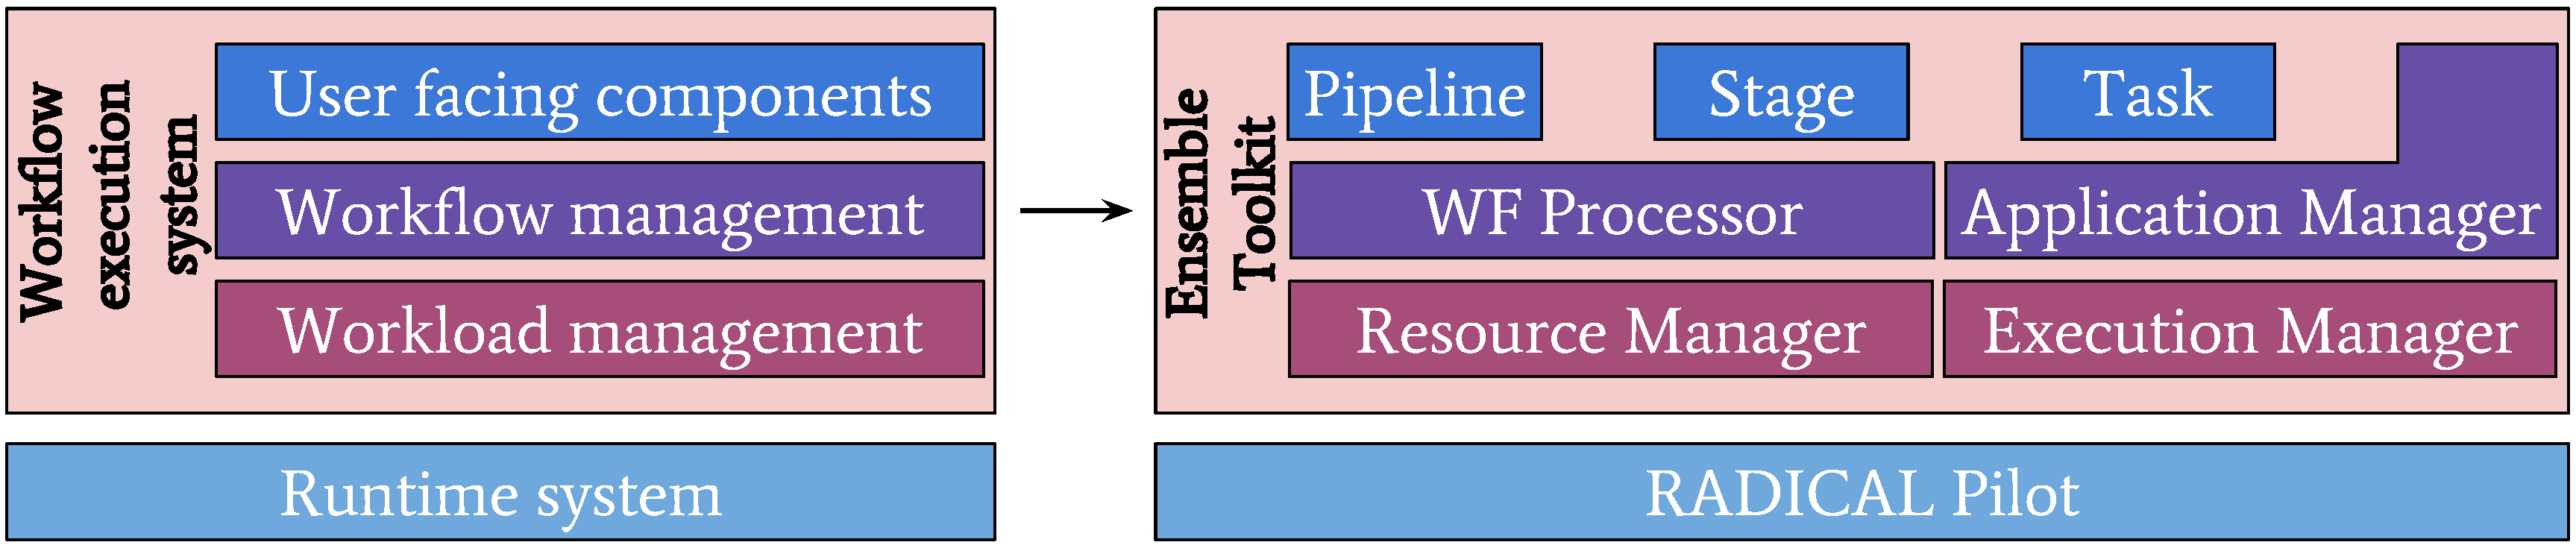
\includegraphics[width=\textwidth, height=35mm]{FIGURES/entk_overview.pdf}
% %  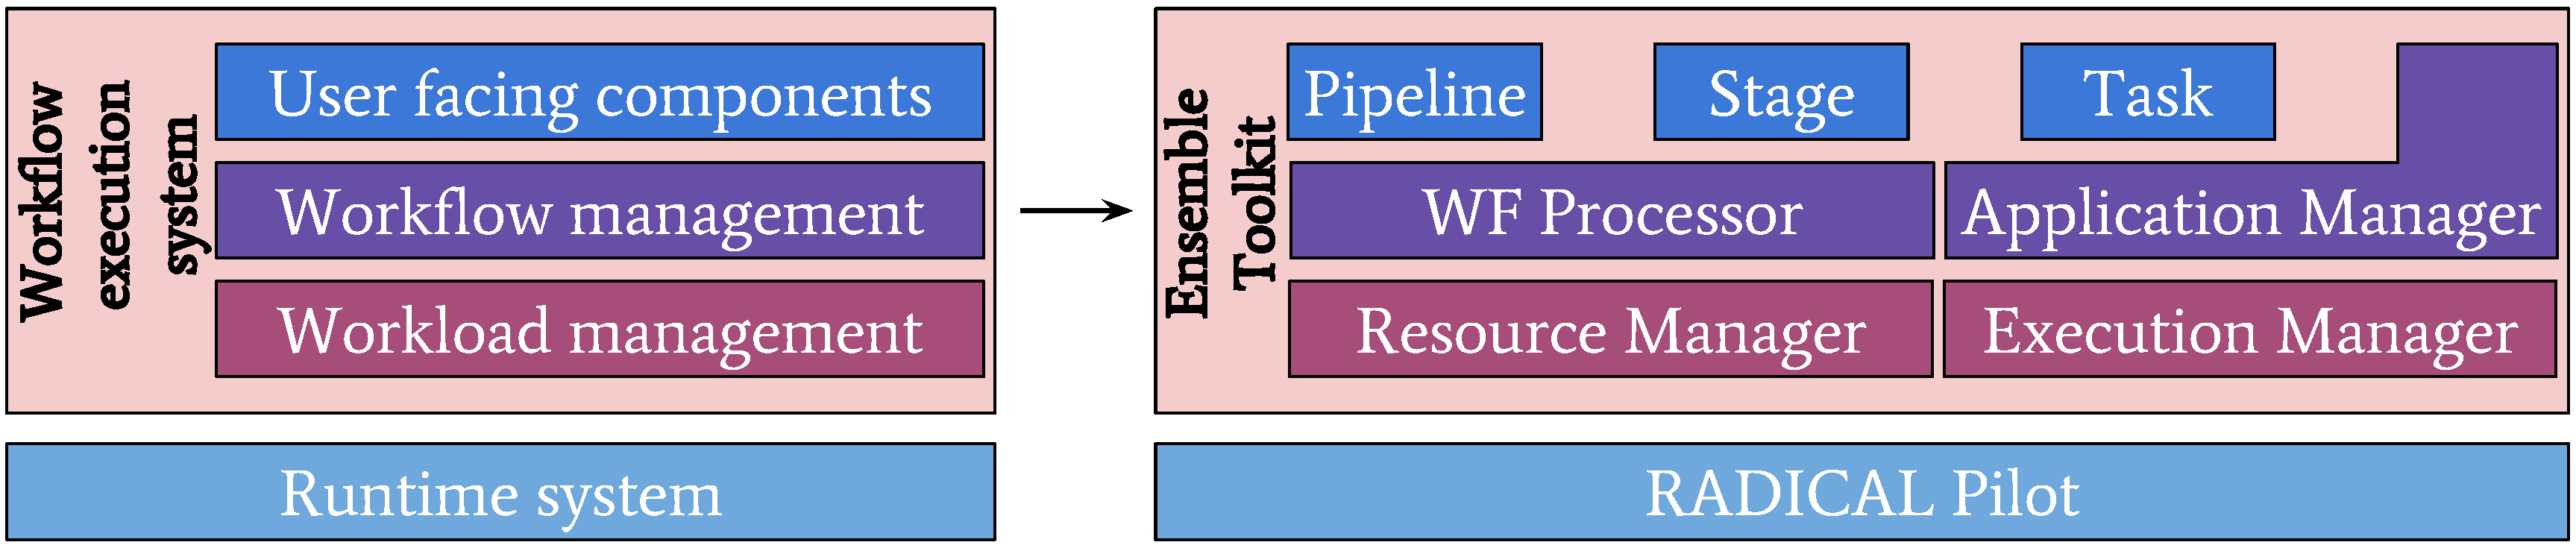
\includegraphics[width=\textwidth, height=40mm]{FIGURES/entk_overview.pdf}
%   \end{minipage}
%   %\begin{minipage}[b]{0.39\textwidth}
%   \begin{minipage}[b]{0.44\textwidth}
%   \centering
% %  \includegraphics[width=\textwidth, height=35mm]{FIGURES/md_general.pdf}
% %  \includegraphics[width=\textwidth, height=40mm]{FIGURES/md_general.pdf}
%   \end{minipage}
%   \caption{Overview of time-to-execution (Tx) of each pipeline at the
%            longest simulation duration as measured by NAMD log files,
%            showing how the distribution shows no abnormal fluctuations
%            across pipelines.}\label{fig:namd_logs}
% \end{figure}

% \begin{figure}[!htbp]
%   \begin{minipage}[b]{0.49\textwidth}
%   \centering
%   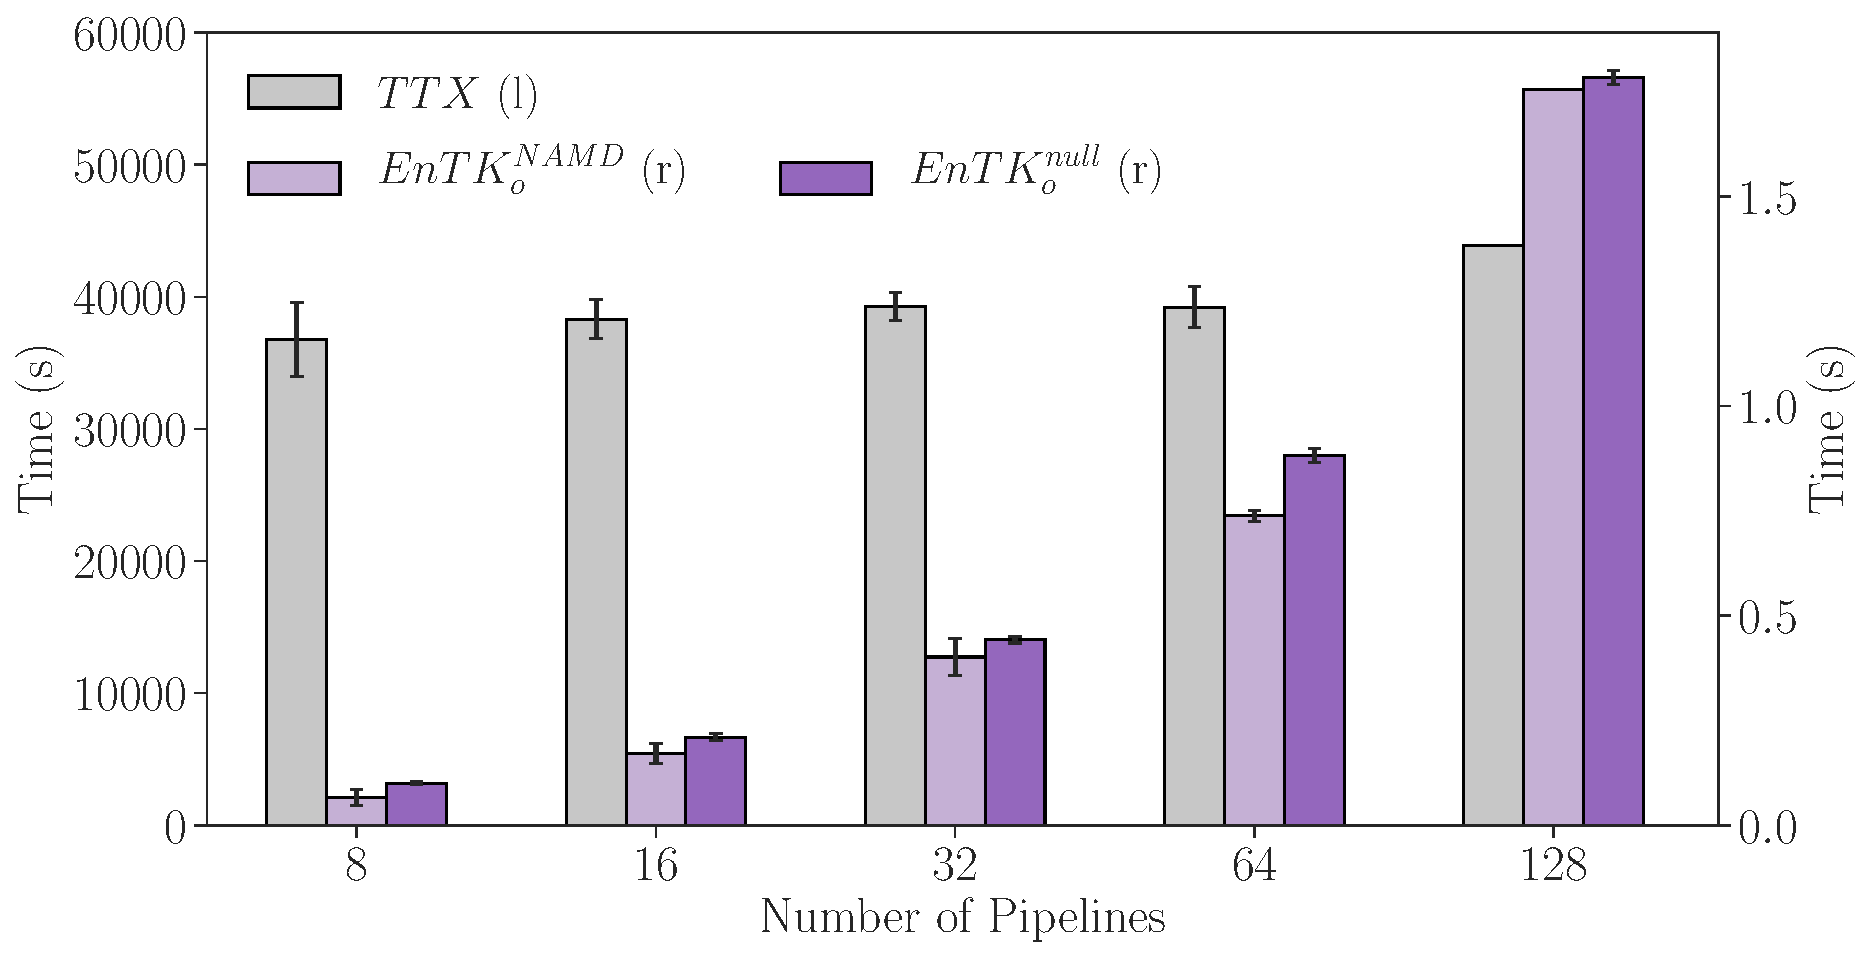
\includegraphics[width=\textwidth]{FIGURES/namd_null_workload_overheads.pdf}
%   \end{minipage}
%   \caption{EnTK overheads for null and NAMD workflows; no pilot overheads.}\label{fig:namd_logs}
% \end{figure}


% NAMD logs - corrolate the overhead for each pipeline makes the system
% invariant to the worload. Remaining will be RP overhead. NAMD log files
% (utime) demonstrates time-to-execution (Tx)

%Add in: what are the overheads, how is EnTK collecting overhead 




%eq0 : Minimize with decreasing restraints
%eq1 : NVT, 50K, with restraints
%eq2 : NPT, 300K, with decreasing restraints 
%sim1.conf: NPT, 300k, no constraints


%Need system verification of timestamps (errors) 







% ---------------------------------------------------------------------------
% VII - CONCLUSION
% ---------------------------------------------------------------------------
%\vspace{-0.1in}
\section{Discussion and Conclusion}\label{sec:conclusion}

It is necessary to move beyond the prevailing paradigm of running individual
MD simulations, which provide irreproducible results and cannot provide
meaningful error bars~\cite{Bhati2017}. Further, the ability to flexibly
scale and adapt ensemble-based protocols to the systems of interest is vital
to produce reliable and accurate results on timescales which make it viable
to influence real world decision making. To meet these goals, we are
designing and developing the high-throughput binding affinity calculator
(HTBAC).

HTBAC employs the RADICAL-Cybertools to build ensemble-based applications for
executing protocols like ESMACS at scale. We show how the implementation of
the ESMACS protocol scales almost perfectly to hundreds of concurrent
pipelines of binding affinity calculations on Blue Waters. 
This permits a time-to-solution that is essentially invariant of the size
of candidate ligands, as well as the type and number of protocols concurrently employed.

% \jhanote{Careful not to imply that HTBAC is a workflow system.}
% \jdnote{better?}\mtnote{Further iterated. Please review.}

% \mtnote{I struggle to understand `This permits the rapid time-to-solution
% that is'} \jdnote{just reduced it to time-to-solution instead of rapid
% time- to-solution}

The use of software implementing well-defined abstractions like that of
``building blocks'', future proofs users of HTBAC to evolving hardware
platforms, while providing immediate benefits of scale and support for a
range of different application workflows. Thus, HTBAC represents an important
advance towards the use of molecular dynamics based free energy calculations
to the point where they can produce actionable results both in the clinic and
industrial drug discovery.

In the short term, the development of HTBAC will allow a significant increase
in the size of study. Much of the literature on MD-based free energy
calculations is limited to a few tens of systems, usually of similar drugs
bound to the same protein target. By facilitating investigations of much
larger datasets, HTBAC also provides a step towards tackling grand challenges
in drug design and precision medicine, where it is necessary to understand
the influences on binding strength for hundreds or thousands of drug-protein
variant combinations. Only in aiming to meet this ambitious goals we will be
able to reveal the limits of existing simulation technology and the
potentials used to approximate the chemistry of the real systems.

\footnotesize \textbf{Software and Data} HTBAC, Ensemble Toolkit and
RADICAL-Pilot can be found respectively at:
\url{https://github.com/radical-cybertools/htbac},
\url{https://github.com/radical-cybertools/radical.entk}, and
\url{https://github.com/radical-cybertools/radical.pilot}. Raw data and
scripts to reproduce experiments can be found at:
\url{https://github.com/radical-experiments/htbac-experiments.}

% \mtnote{Should we add a link to HTBAC code base?}
% \jdnote{Not sure, in case yes, }



% ---------------------------------------------------------------------------
% ACKNOWLEDGEMENTS
% ---------------------------------------------------------------------------
\section*{Acknowledgements}

\footnotesize

Access to Blue Waters was made possible by NSF OAC 1713749. The software
capabilities were supported by RADICAL-Cybertools (OAC 1440677) and NSF ICER
1639694. We thank Andre Merzky and other members of the RADICAL team for
support. PVC, SJZ and DWW would like to acknowledge the support of the EU
H2020 CompBioMed (675451), EUDAT2020 (654065) and ComPat (671564) projects. 
We acknowledge MRC Medical Bioinformatics project (MR/ L016311/1), 
and funding from the UCL Provost. 

{\it Author Roles and Contribution:} PVC and SJ conceived this work. MT and SJ
designed the experiments with support from JD and VB. JD performed the bulk of
experiments on Blue Waters, with support from DWW and VB. VB developed the
version of EnTK used for experiments. MT, VB, JD and SJ analyzed the data. SJZ
initially developed the ESMACS protocol using EnTK. DWW, MT and SJ wrote the
bulk of the paper.

HTBAC, Ensemble Toolkit and
RADICAL-Pilot can be found respectively at:
\url{https://github.com/radical-cybertools/htbac},
\url{https://github.com/radical-cybertools/radical.entk}, and
\url{https://github.com/radical-cybertools/radical.pilot}. Raw data and
scripts to reproduce experiments can be found at:
\url{https://github.com/radical-experiments/htbac-experiments.}


% Vivek Balasubramanian,

% Dave Wright,

% Stefan Zasada, Matteo Turilli

% Shunzhou Wan



% Peter V. Coveney
% Shantenu Jha



% ---------------------------------------------------------------------------
% REFERENCES
% ---------------------------------------------------------------------------
\bibliographystyle{IEEEtran}
\bibliography{rutgers,ucl}

\end{document}